%==============================================================================
% tento soubor pouzijte jako zaklad
% this file should be used as a base for the thesis
% Autoři / Authors: 2008 Michal Bidlo, 2016 Jaroslav Dytrych


% Kontakt pro dotazy a připomínky: dytrych@fit.vutbr.cz
% Contact for questions and comments: dytrych@fit.vutbr.cz
%==============================================================================
% kodovaní: UTF-8 (zmena prikazem iconv, recode nebo cstocs)
% encoding: UTF-8 (you can change it by command iconv, recode or cstocs)
%------------------------------------------------------------------------------
% zpracování / processing: make, make pdf, make clean
%==============================================================================
% Soubory, které je nutné upravit: / Files which have to be edited:
%   projekt-20-literatura-bibliography.bib - literatura / bibliography
%   projekt-01-kapitoly-chapters.tex - obsah práce / the thesis content
%   projekt-30-prilohy-appendices.tex - přílohy / appendices
%==============================================================================
\documentclass[]{fitthesis} % bez zadání - pro začátek práce, aby nebyl problém s překladem
%\documentclass[english]{fitthesis} % without assignment - for the work start to avoid compilation problem
%\documentclass[zadani]{fitthesis} % odevzdani do wisu - odkazy jsou barevné
%\documentclass[english,zadani]{fitthesis} % for submission to the IS FIT - links are color
%\documentclass[zadani,print]{fitthesis} % pro tisk - odkazy jsou černé
%\documentclass[english,zadani,print]{fitthesis} % for the print - links are black
% * Je-li prace psana v anglickem jazyce, je zapotrebi u tridy pouzit 
%   parametr english nasledovne:
%   If thesis is written in english, it is necessary to use 
%   parameter english as follows:
%      \documentclass[english]{fitthesis}
% * Je-li prace psana ve slovenskem jazyce, je zapotrebi u tridy pouzit 
%   parametr slovak nasledovne:
%      \documentclass[slovak]{fitthesis}

% Základní balíčky jsou dole v souboru šablony fitthesis.cls
% Basic packages are at the bottom of template file fitthesis.cls

%zde muzeme vlozit vlastni balicky / you can place own packages here
%footnote in caption for figure
\usepackage{graphicx}
\usepackage{afterpage}

%subfigure
\usepackage{caption}
\usepackage{subcaption}

%---rm---------------
\renewcommand{\rmdefault}{lmr}%zavede Latin Modern Roman jako rm / set Latin Modern Roman as rm
%---sf---------------
\renewcommand{\sfdefault}{qhv}%zavede TeX Gyre Heros jako sf
%---tt------------
\renewcommand{\ttdefault}{lmtt}% zavede Latin Modern tt jako tt

% vypne funkci šablony, která automaticky nahrazuje uvozovky,
% aby nebyly prováděny nevhodné náhrady v popisech API apod.
% disables function of the template which replaces quotation marks
% to avoid unnecessary replacements in the API descriptions etc.
\csdoublequotesoff

% =======================================================================
% balíček "hyperref" vytváří klikací odkazy v pdf, pokud tedy použijeme pdflatex
% problém je, že balíček hyperref musí být uveden jako poslední, takže nemůže
% být v šabloně
% "hyperref" package create clickable links in pdf if you are using pdflatex.
% Problem is that this package have to be introduced as the last one so it 
% can not be placed in the template file.
\ifWis
\ifx\pdfoutput\undefined % nejedeme pod pdflatexem / we are not using pdflatex
\else
  \usepackage{color}
  \usepackage[unicode,colorlinks,hyperindex,plainpages=false,pdftex]{hyperref}
  \definecolor{links}{rgb}{0.4,0.5,0}
  \definecolor{anchors}{rgb}{1,0,0}
  \def\AnchorColor{anchors}
  \def\LinkColor{links}
  \def\pdfBorderAttrs{/Border [0 0 0] }  % bez okrajů kolem odkazů / without margins around links
  \pdfcompresslevel=9
\fi
\else % pro tisk budou odkazy, na které se dá klikat, černé / for the print clickable links will be black
\ifx\pdfoutput\undefined % nejedeme pod pdflatexem / we are not using pdflatex
\else
  \usepackage{color}
  \usepackage[unicode,colorlinks,hyperindex,plainpages=false,pdftex,urlcolor=black,linkcolor=black,citecolor=black]{hyperref}
  \definecolor{links}{rgb}{0,0,0}
  \definecolor{anchors}{rgb}{0,0,0}
  \def\AnchorColor{anchors}
  \def\LinkColor{links}
  \def\pdfBorderAttrs{/Border [0 0 0] } % bez okrajů kolem odkazů / without margins around links
  \pdfcompresslevel=9
\fi
\fi
% Řešení problému, kdy klikací odkazy na obrázky vedou za obrázek
% This solves the problems with links which leads after the picture
\usepackage[all]{hypcap}

% Informace o práci/projektu / Information about the thesis
%---------------------------------------------------------------------------
\projectinfo{
  %Prace / Thesis
  project=SP,            %typ prace BP/SP/DP/DR  / thesis type (SP = term project)
  year=2017,             %rok odevzdání / year of submission
  date=\today,           %datum odevzdani / submission date
  %Nazev prace / thesis title
  title.cs={
Lego Mindstorm EV3 ve výuce programování a robotiky},  %nazev prace v cestine ci slovenstine (dle zadani) / thesis title in czech language (according to assignment)
  title.en={Lego Mindstorm EV3 in Education of Programming and Robotics}, %nazev prace v anglictine / thesis title in english
  %Autor / Author
  author={Jaroslav Páral},   %cele jmeno a prijmeni autora / full name and surname of the author
  author.name={Jaroslav},   %jmeno autora (pro citaci) / author name (for reference) 
  author.surname={Páral},   %prijmeni autora (pro citaci) / author surname (for reference) 
  %author.title.p=Bc., %titul pred jmenem (nepovinne) / title before the name (optional)
  %author.title.a=PhD, %titul za jmenem (nepovinne) / title after the name (optional)
  %Ustav / Department
  department=UITS, % doplnte prislusnou zkratku dle ustavu na zadani: UPSY/UIFS/UITS/UPGM
  %                  fill in appropriate abbreviation of the department according to assignment: UPSY/UIFS/UITS/UPGM
  %Skolitel / supervisor
  supervisor={Filip Orság}, %cele jmeno a prijmeni skolitele / full name and surname of the supervisor
  supervisor.name={Filip},   %jmeno skolitele (pro citaci) / supervisor name (for reference) 
  supervisor.surname={Orság},   %prijmeni skolitele (pro citaci) / supervisor surname (for reference) 
  supervisor.title.p=Ing.,   %titul pred jmenem (nepovinne) / title before the name (optional)
  supervisor.title.a={Ph.D.},    %titul za jmenem (nepovinne) / title after the name (optional)
  %Klicova slova, abstrakty, prohlaseni a podekovani je mozne definovat 
  %bud pomoci nasledujicich parametru nebo pomoci vyhrazenych maker (viz dale)
  %Keywords, abstracts, declaration and acknowledgement can be defined by following 
  %parameters or using dedicated macros (see below)
  %===========================================================================
  %Klicova slova / keywords
  %keywords.cs={Klíčová slova v českém jazyce.}, %klicova slova v ceskem ci slovenskem jazyce
  %                                              keywords in czech or slovak language
  %keywords.en={Klíčová slova v anglickém jazyce.}, %klicova slova v anglickem jazyce / keywords in english
  %Abstract
  %abstract.cs={Výtah (abstrakt) práce v českém jazyce.}, % abstrakt v ceskem ci slovenskem jazyce
  %                                                         abstract in czech or slovak language
  %abstract.en={Výtah (abstrakt) práce v anglickém jazyce.}, % abstrakt v anglickem jazyce / abstract in english
  %Prohlaseni / Declaration
  %declaration={Prohlašuji, že jsem tuto bakalářskou práci vypracoval samostatně pod vedením pana ...},
  %Podekovani (nepovinne) / Acknowledgement (optional)
  %acknowledgment={Zde je možné uvést poděkování vedoucímu práce a těm, kteří poskytli odbornou pomoc.} % nepovinne
  %acknowledgment={Here it is possible to express thanks to the supervisor and to the people which provided professional help.} % optional
}

% Definice vlastních maker / own macros

\newcommand{\lego}{LEGO}
\newcommand{\lega}{LEGA}
\newcommand{\legoM}{LEGO MINDSTORMS}
\newcommand{\legoNXT}{LEGO MINDSTORMS NXT}
\newcommand{\legoEV}{LEGO MINDSTORMS EV3}
\newcommand{\EVthree}{EV3}


\newcommand{\fll}{{\it FIRST} LEGO League}
\newcommand{\brick}{{\it Brick}}

\newcommand{\evThreeDev}{{\it ev3dev}}
\newcommand{\leJOS}{{leJOS}}

\newcommand{\NI}{National Instruments}
\newcommand{\labview}{LabVIEW}

\newcommand{\fischerT}{{\it fischertechnik}}
\newcommand{\FischerT}{{\it Fischertechnik}}

\newcommand{\merkur}{Merkur}

\newcommand{\arduino}{Arduino}



%Abstrakt (cesky, slovensky ci anglicky) / Abstract (in czech, slovak or english)
\abstract[cs]{Cílem této práce je srovnat vývojové platformy pro stavebnici \legoEV{ }z pohledu programování a nejlepšího využití v rámci robotiky. Proto jsou hlavními srovnávacími parametry výkonnost, náročnost programování při rozsáhlejších projektech a propojení %propojení/spojitost/spojení 
s běžnými programovacími jazyky (C/C++, Java, Python, \ldots). 
V práci není kladen hlavní důraz na výběr nejvhodnější platformy pro úplné začátečníky v programování. % s LEGO MINDSTORMS?
Naopak primárním úkolem je najít vhodnou platformu pro lidi, kterým již standardní vývojové prostředí dodávané se stavebnicí nedostačuje a hledají lepší alternativu. }
\abstract[en]{Do tohoto odstavce bude zapsán výtah (abstrakt) práce v anglickém jazyce.}

%Klicova slova (cesky, slovensky ci anglicky) / Keywords (in czech, slovak or english)
\keywords[cs]{\legoEV, programovací platformy, ev3dev, LeJOS, ROS, Matlab, EV3RT, ROBOTC}
\keywords[en]{\legoEV, programing platforms, ev3dev, LeJOS, ROS, Matlab, EV3RT, ROBOTC}

%Prohlaseni (u anglicky psane prace anglicky, u slovensky psane prace slovensky)
%Declaration (for thesis in english should be in english)
\declaration{Prohlašuji, že jsem tuto bakalářskou práci vypracoval samostatně pod vedením pana Ing.~Filipa Orsága, Ph.D.
Uvedl jsem všechny literární prameny a publikace, ze kterých jsem čerpal.}

% \declaration{Hereby I declare that this bachelor's thesis was prepared as an original author’s work under the supervision of Mr. X
% The supplementary information was provided by Mr. Y
% All the relevant information sources, which were used during preparation of this thesis, are properly cited and included in the list of references.}

%Podekovani (nepovinne, nejlepe v jazyce prace) / Acknowledgement (optional, ideally in the language of the thesis)
\acknowledgment{V této sekci je možno uvést poděkování vedoucímu práce a těm, kteří poskytli odbornou pomoc
(externí zadavatel, konzultant, apod.).}
%\acknowledgment{Here it is possible to express thanks to the supervisor and to the people which provided professional help
%(external submitter, consultant, etc.).}

% řeší první/poslední řádek odstavce na předchozí/následující stránce
% solves first/last row of the paragraph on the previous/next page
\clubpenalty=10000
\widowpenalty=10000

\begin{document}
  % Vysazeni titulnich stran / Typesetting of the title pages
  % ----------------------------------------------
  \maketitle
  % Obsah
  % ----------------------------------------------
  \setlength{\parskip}{0pt}

  {\hypersetup{hidelinks}\tableofcontents}
  
  % Seznam obrazku a tabulek (pokud prace obsahuje velke mnozstvi obrazku, tak se to hodi)
  % List of figures and list of tables (if the thesis contains a lot of pictures, it is good)
  \ifczech
    \renewcommand\listfigurename{Seznam obrázků}
  \fi
  \ifslovak
    \renewcommand\listfigurename{Zoznam obrázkov}
  \fi

  \listoffigures

  
  \ifczech
    \renewcommand\listtablename{Seznam tabulek}
  \fi
  \ifslovak
    \renewcommand\listtablename{Zoznam tabuliek}
  \fi

  % \listoftables 

  \ifODSAZ
    \setlength{\parskip}{0.5\bigskipamount}
  \else
    \setlength{\parskip}{0pt}
  \fi

  % vynechani stranky v oboustrannem rezimu
  % Skip the page in the two-sided mode
  \iftwoside
    \cleardoublepage
  \fi
  % Text prace / Thesis text
  % ----------------------------------------------
  %%=========================================================================
% (c) Michal Bidlo, Bohuslav Křena, 2008

\chapter{Úvod}
Abychom mohli napsat odborný text jasně a~srozumitelně, musíme splnit několik základních předpokladů:
\begin{itemize}
\item Musíme mít co říci,
\item musíme vědět, komu to chceme říci,
\item musíme si dokonale promyslet obsah,
\item musíme psát strukturovaně. 
\end{itemize}

Tyto a další pokyny jsou dostupné též na školních internetových stránkách \cite{fitWeb}.

Přehled základů typografie a tvorby dokumentů s využitím systému \LaTeX je 
uveden v~\cite{Rybicka}.

\section{Musíme mít co říci}
Dalším důležitým předpokladem dobrého psaní je {\it psát pro někoho}. Píšeme-li si poznámky sami pro sebe, píšeme je jinak než výzkumnou zprávu, článek, diplomovou práci, knihu nebo dopis. Podle předpokládaného čtenáře se rozhodneme pro způsob psaní, rozsah informace a~míru detailů.

\section{Musíme vědět, komu to chceme říci}
Dalším důležitým předpokladem dobrého psaní je psát pro někoho. Píšeme-li si poznámky sami pro sebe, píšeme je jinak než výzkumnou zprávu, článek, diplomovou práci, knihu nebo dopis. Podle předpokládaného čtenáře se rozhodneme pro způsob psaní, rozsah informace a~míru detailů.

\section{Musíme si dokonale promyslet obsah}
Musíme si dokonale promyslet a~sestavit obsah sdělení a~vytvořit pořadí, v~jakém chceme čtenáři své myšlenky prezentovat. 
Jakmile víme, co chceme říci a~komu, musíme si rozvrhnout látku. Ideální je takové rozvržení, které tvoří logicky přesný a~psychologicky stravitelný celek, ve kterém je pro všechno místo a~jehož jednotlivé části do sebe přesně zapadají. Jsou jasné všechny souvislosti a~je zřejmé, co kam patří.

Abychom tohoto cíle dosáhli, musíme pečlivě organizovat látku. Rozhodneme, co budou hlavní kapitoly, co podkapitoly a~jaké jsou mezi nimi vztahy. Diagramem takové organizace je graf, který je velmi podobný stromu, ale ne řetězci. Při organizaci látky je stejně důležitá otázka, co do osnovy zahrnout, jako otázka, co z~ní vypustit. Příliš mnoho podrobností může čtenáře právě tak odradit jako žádné detaily.

Výsledkem této etapy je osnova textu, kterou tvoří sled hlavních myšlenek a~mezi ně zařazené detaily.

\section{Musíme psát strukturovaně} 
Musíme začít psát strukturovaně a~současně pracujeme na co nejsrozumitelnější formě, včetně dobrého slohu a~dokonalého značení. 
Máme-li tedy myšlenku, představu o~budoucím čtenáři, cíl a~osnovu textu, můžeme začít psát. Při psaní prvního konceptu se snažíme zaznamenat všechny své myšlenky a~názory vztahující se k~jednotlivým kapitolám a~podkapitolám. Každou myšlenku musíme vysvětlit, popsat a~prokázat. Hlavní myšlenku má vždy vyjadřovat hlavní věta a~nikoliv věta vedlejší.

I k~procesu psaní textu přistupujeme strukturovaně. Současně s~tím, jak si ujasňujeme strukturu písemné práce, vytváříme kostru textu, kterou postupně doplňujeme. Využíváme ty prostředky DTP programu, které podporují strukturovanou stavbu textu (předdefinované typy pro nadpisy a~bloky textu). 


\chapter{Několik formálních pravidel}
Naším cílem je vytvořit jasný a~srozumitelný text. Vyjadřujeme se proto přesně, píšeme dobrou češtinou (nebo zpravidla angličtinou) a~dobrým slohem podle obecně přijatých zvyklostí. Text má upravit čtenáři cestu k~rychlému pochopení problému, předvídat jeho obtíže a~předcházet jim. Dobrý sloh předpokládá bezvadnou gramatiku, správnou interpunkci a~vhodnou volbu slov. Snažíme se, aby náš text nepůsobil příliš jednotvárně používáním malého výběru slov a~tím, že některá zvlášť oblíbená slova používáme příliš často. Pokud používáme cizích slov, je samozřejmým předpokladem, že známe jejich přesný význam. Ale i~českých slov musíme používat ve správném smyslu. Např. platí jistá pravidla při používání slova {\it zřejmě}. Je {\it zřejmé} opravdu zřejmé? A~přesvědčili jsme se, zda to, co je {\it zřejmé} opravdu platí? Pozor bychom si měli dát i~na příliš časté používání zvratného se. Například obratu {\it dokázalo se}, že... zásadně nepoužíváme. Není špatné používat autorského {\it my}, tím předpokládáme, že něco řešíme, nebo například zobecňujeme spolu se čtenářem. V~kvalifikačních pracích použijeme autorského {\it já} (například když vymezujeme podíl vlastní práce vůči převzatému textu), ale v~běžném textu se nadměrné používání první osoby jednotného čísla nedoporučuje.

Za pečlivý výběr stojí i~symbolika, kterou používáme ke {\it značení}. Máme tím na mysli volbu zkratek a~symbolů používaných například pro vyjádření typů součástek, pro označení hlavních činností programu, pro pojmenování ovládacích kláves na klávesnici, pro pojmenování proměnných v~matematických formulích a~podobně. Výstižné a~důsledné značení může čtenáři při četbě textu velmi pomoci. Je vhodné uvést seznam značení na začátku textu. Nejen ve značení, ale i~v~odkazech a~v~celkové tiskové úpravě je důležitá důslednost.

S tím souvisí i~pojem z~typografie nazývaný {\it vyznačování}. Zde máme na mysli způsob sazby textu pro jeho zvýraznění. Pro zvolené značení by měl být zvolen i~způsob vyznačování v~textu. Tak například klávesy mohou být umístěny do obdélníčku, identifikátory ze zdrojového textu mohou být vypisovány {\tt písmem typu psací stroj} a~podobně.

Uvádíme-li některá fakta, neskrýváme jejich původ a~náš vztah k~nim. Když něco tvrdíme, vždycky výslovně uvedeme, co z~toho bylo dokázáno, co teprve bude dokázáno v~našem textu a~co přebíráme z~literatury s~uvedením odkazu na příslušný zdroj. V~tomto směru nenecháváme čtenáře nikdy na pochybách, zda jde o~myšlenku naši nebo převzatou z~literatury.

Nikdy neplýtváme čtenářovým časem výkladem triviálních a~nepodstatných informací. Neuvádíme rovněž několikrát totéž jen jinými slovy. Při pozdějších úpravách textu se nám může některá dříve napsaná pasáž jevit jako zbytečně podrobná nebo dokonce zcela zbytečná. Vypuštění takové pasáže nebo alespoň její zestručnění přispěje k~lepší čitelnosti práce! Tento krok ale vyžaduje odvahu zahodit čas, který jsme jejímu vytvoření věnovali. 


\chapter{Nikdy to nebude naprosto dokonalé}
Když jsme už napsali vše, o~čem jsme přemýšleli, uděláme si den nebo dva dny volna a~pak si přečteme sami rukopis znovu. Uděláme ještě poslední úpravy a~skončíme. Jsme si vědomi toho, že vždy zůstane něco nedokončeno, vždy existuje lepší způsob, jak něco vysvětlit, ale každá etapa úprav musí být konečná.


\chapter{Typografické a~jazykové zásady}
Při tisku odborného textu typu {\it technická zpráva} (anglicky {\it technical report}), ke kterému patří například i~text kvalifikačních prací, se často volí formát A4 a~často se tiskne pouze po jedné straně papíru. V~takovém případě volte levý okraj všech stránek o~něco větší než pravý -- v~tomto místě budou papíry svázány a~technologie vazby si tento požadavek vynucuje. Při vazbě s~pevným hřbetem by se levý okraj měl dělat o~něco širší pro tlusté svazky, protože se stránky budou hůře rozevírat a~levý okraj se tak bude oku méně odhalovat.

Horní a~spodní okraj volte stejně veliký, případně potištěnou část posuňte mírně nahoru (horní okraj menší než dolní). Počítejte s~tím, že při vazbě budou okraje mírně oříznuty.

Pro sazbu na stránku formátu A4 je vhodné používat pro základní text písmo stupně (velikosti) 11 bodů. Volte šířku sazby 15 až 16 centimetrů a~výšku 22 až 23 centimetrů (včetně případných hlaviček a~patiček). Proklad mezi řádky se volí 120 procent stupně použitého základního písma, což je optimální hodnota pro rychlost čtení souvislého textu. V~případě použití systému LaTeX ponecháme implicitní nastavení. Při psaní kvalifikační práce se řiďte příslušnými závaznými požadavky.

Stupeň písma u~nadpisů různé úrovně volíme podle standardních typografických pravidel. 
Pro všechny uvedené druhy nadpisů se obvykle používá polotučné nebo tučné písmo (jednotně buď všude polotučné nebo všude tučné). Proklad se volí tak, aby se následující text běžných odstavců sázel pokud možno na {\it pevný rejstřík}, to znamená jakoby na linky s~předem definovanou a~pevnou roztečí.

Uspořádání jednotlivých částí textu musí být přehledné a~logické. Je třeba odlišit názvy kapitol a~podkapitol -- píšeme je malými písmeny kromě velkých začátečních písmen. U~jednotlivých odstavců textu odsazujeme první řádek odstavce asi o~jeden až dva čtverčíky (vždy o~stejnou, předem zvolenou hodnotu), tedy přibližně o~dvě šířky velkého písmene M základního textu. Poslední řádek předchozího odstavce a~první řádek následujícího odstavce se v~takovém případě neoddělují svislou mezerou. Proklad mezi těmito řádky je stejný jako proklad mezi řádky uvnitř odstavce.

Při vkládání obrázků volte jejich rozměry tak, aby nepřesáhly oblast, do které se tiskne text (tj. okraje textu ze všech stran). Pro velké obrázky vyčleňte samostatnou stránku. Obrázky nebo tabulky o~rozměrech větších než A4 umístěte do písemné zprávy formou skládanky všité do přílohy nebo vložené do záložek na zadní desce.

Obrázky i~tabulky musí být pořadově očíslovány. Číslování se volí buď průběžné v~rámci celého textu, nebo -- což bývá praktičtější -- průběžné v~rámci kapitoly. V~druhém případě se číslo tabulky nebo obrázku skládá z~čísla kapitoly a~čísla obrázku/tabulky v~rámci kapitoly -- čísla jsou oddělena tečkou. Čísla podkapitol nemají na číslování obrázků a~tabulek žádný vliv.

Tabulky a~obrázky používají své vlastní, nezávislé číselné řady. Z toho vyplývá, že v~odkazech uvnitř textu musíme kromě čísla udat i~informaci o~tom, zda se jedná o~obrázek či tabulku (například ``... {\it viz tabulka 2.7} ...''). Dodržování této zásady je ostatně velmi přirozené.

Pro odkazy na stránky, na čísla kapitol a~podkapitol, na čísla obrázků a~tabulek a~v~dalších podobných příkladech využíváme speciálních prostředků DTP programu, které zajistí vygenerování správného čísla i~v~případě, že se text posune díky změnám samotného textu nebo díky úpravě parametrů sazby. Příkladem takového prostředku v~systému LaTeX je odkaz na číslo odpovídající umístění značky v~textu, například návěští ($\backslash${\tt ref\{navesti\}} -- podle umístění návěští se bude jednat o~číslo kapitoly, podkapitoly, obrázku, tabulky nebo podobného číslovaného prvku), na stránku, která obsahuje danou značku ($\backslash${\tt pageref\{navesti\}}), nebo na literární odkaz ($\backslash${\tt cite\{identifikator\}}).

Rovnice, na které se budeme v~textu odvolávat, opatříme pořadovými čísly při pravém okraji příslušného řádku. Tato pořadová čísla se píší v~kulatých závorkách. Číslování rovnic může být průběžné v~textu nebo v~jednotlivých kapitolách.

Jste-li na pochybách při sazbě matematického textu, snažte se dodržet způsob sazby definovaný systémem LaTeX. Obsahuje-li vaše práce velké množství matematických formulí, doporučujeme dát přednost použití systému LaTeX.

Mezeru neděláme tam, kde se spojují číslice s~písmeny v~jedno slovo nebo v~jeden znak -- například {\it 25krát}.

Členicí (interpunkční) znaménka tečka, čárka, středník, dvojtečka, otazník a~vykřičník, jakož i~uzavírací závorky a~uvozovky se přimykají k~předcházejícímu slovu bez mezery. Mezera se dělá až za nimi. To se ovšem netýká desetinné čárky (nebo desetinné tečky). Otevírací závorka a~přední uvozovky se přimykají k~následujícímu slovu a~mezera se vynechává před nimi -- (takto) a~``takto''.

Pro spojovací a~rozdělovací čárku a~pomlčku nepoužíváme stejný znak. Pro pomlčku je vyhrazen jiný znak (delší). V~systému TeX (LaTeX) se spojovací čárka zapisuje jako jeden znak ``pomlčka'' (například ``Brno-město''), pro sázení textu ve smyslu intervalu nebo dvojic, soupeřů a~podobně se ve zdrojovém textu používá dvojice znaků ``pomlčka'' (například ``zápas Sparta -- Slavie''; ``cena 23--25 korun''), pro výrazné oddělení části věty, pro výrazné oddělení vložené věty, pro vyjádření nevyslovené myšlenky a~v~dalších situacích (viz Pravidla českého pravopisu) se používá nejdelší typ pomlčky, která se ve zdrojovém textu zapisuje jako trojice znaků ``pomlčka'' (například ``Další pojem --- jakkoliv se může zdát nevýznamný --- bude neformálně definován v~následujícím odstavci.''). Při sazbě matematického mínus se při sazbě používá rovněž odlišný znak. V~systému TeX je ve zdrojovém textu zapsán jako normální mínus (tj. znak ``pomlčka''). Sazba v~matematickém prostředí, kdy se vzoreček uzavírá mezi dolary, zajistí vygenerování správného výstupu.

Lomítko se píše bez mezer. Například školní rok 2008/2009.

Pravidla pro psaní zkratek jsou uvedena v~Pravidlech českého pravopisu \cite{Pravidla}. I~z~jiných důvodů je vhodné, abyste tuto knihu měli po ruce. 


\section{Co to je normovaná stránka?}
Pojem {\it normovaná stránka} se vztahuje k~posuzování objemu práce, nikoliv k~počtu vytištěných listů. Z historického hlediska jde o~počet stránek rukopisu, který se psal psacím strojem na speciální předtištěné formuláře při dodržení průměrné délky řádku 60 znaků a~při 30 řádcích na stránku rukopisu. Vzhledem k~zápisu korekturních značek se používalo řádkování 2 (ob jeden řádek). Tyto údaje (počet znaků na řádek, počet řádků a~proklad mezi nimi) se nijak nevztahují ke konečnému vytištěnému výsledku. Používají se pouze pro posouzení rozsahu. Jednou normovanou stránkou se tedy rozumí 60*30 = 1800 znaků. Obrázky zařazené do textu se započítávají do rozsahu písemné práce odhadem jako množství textu, které by ve výsledném dokumentu potisklo stejně velkou plochu.

Orientační rozsah práce v~normostranách lze v~programu Microsoft Word zjistit pomocí funkce {\it Počet slov} v~menu {\it Nástroje}, když hodnotu {\it Znaky (včetně mezer)} vydělíte konstantou 1800. Do rozsahu práce se započítává pouze text uvedený v~jádru práce. Části jako abstrakt, klíčová slova, prohlášení, obsah, literatura nebo přílohy se do rozsahu práce nepočítají. Je proto nutné nejdříve označit jádro práce a~teprve pak si nechat spočítat počet znaků. Přibližný rozsah obrázků odhadnete ručně. Podobně lze postupovat i~při použití OpenOffice. Při použití systému LaTeX pro sazbu je situace trochu složitější. Pro hrubý odhad počtu normostran lze využít součet velikostí zdrojových souborů práce podělený konstantou cca 2000 (normálně bychom dělili konstantou 1800, jenže ve zdrojových souborech jsou i~vyznačovací příkazy, které se do rozsahu nepočítají). Pro přesnější odhad lze pak vyextrahovat holý text z~PDF (např. metodou cut-and-paste nebo {\it Save as Text...}) a~jeho velikost podělit konstantou 1800. 


\chapter{Závěr}
Závěrečná kapitola obsahuje zhodnocení dosažených výsledků se zvlášť vyznačeným vlastním přínosem studenta. Povinně se zde objeví i zhodnocení z pohledu dalšího vývoje projektu, student uvede náměty vycházející ze zkušeností s řešeným projektem a uvede rovněž návaznosti na právě dokončené projekty.

%=========================================================================
 % viz. obsah.tex / see obsah.tex		
  
  \chapter{Úvod}

Stavebnice \lego{ }je jedna z~nejznámějších a nejprodávanějších stavebnicí na světě. 

V~nabídce firmy \lego{ }je i~robotický set s~názvem \legoM. 

Dle oficiálních údajů se jedná historicky nejprodávanější set z~celé nabídky firmy~\cite{legoGizmodo_SalesStatistic}. 
To je také jeden z~hlavních důvodů, proč se tato práce věnuje této stavebnici. 
%To je také jeden z hlavních důvodů, proč je tato práce zaměřena na tuto stavebnici. 

Z~výše uvedených informací vyplývá, že jde pravděpodobně o~nejdostupnější robotickou stavebnici na světě (pokud pomineme platformu \arduino, která je ovšem zaměřena na jinou skupinu lidí -- lidí, kteří se nebojí elektroniky, elektronických obvodů, složitějších návrhů konstrukce, atd.).

\begin{figure}[h]
	\centering
	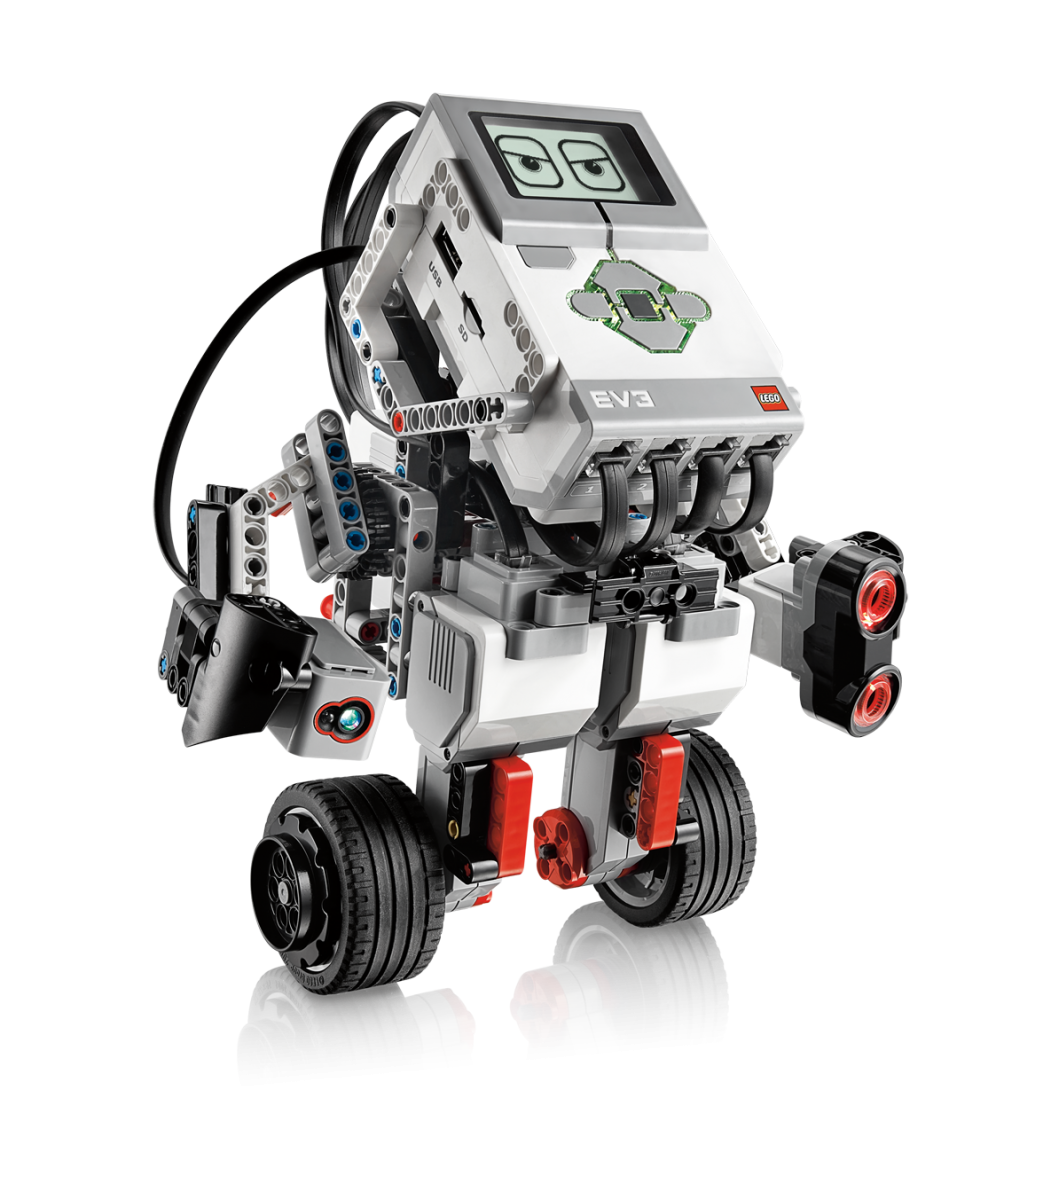
\includegraphics[width=250px]{images/lego-mindstorms-ev3_Robotics-for-Kids.png}
	\caption[\legoEV{ }-- samobalancující robot]{\legoEV{ }-- samobalancující robot\protect\footnotemark}
	\label{fig:lego-mindstorms-ev3_Robotics-for-Kids}
\end{figure}


\footnotetext{Zdroj: \url{https://www.bermotech.com/training/coding-for-teenagers-and-children/y-robotics-with-lego-mindstorm-ev3/}}

\begin{figure}[h]
	\centering
	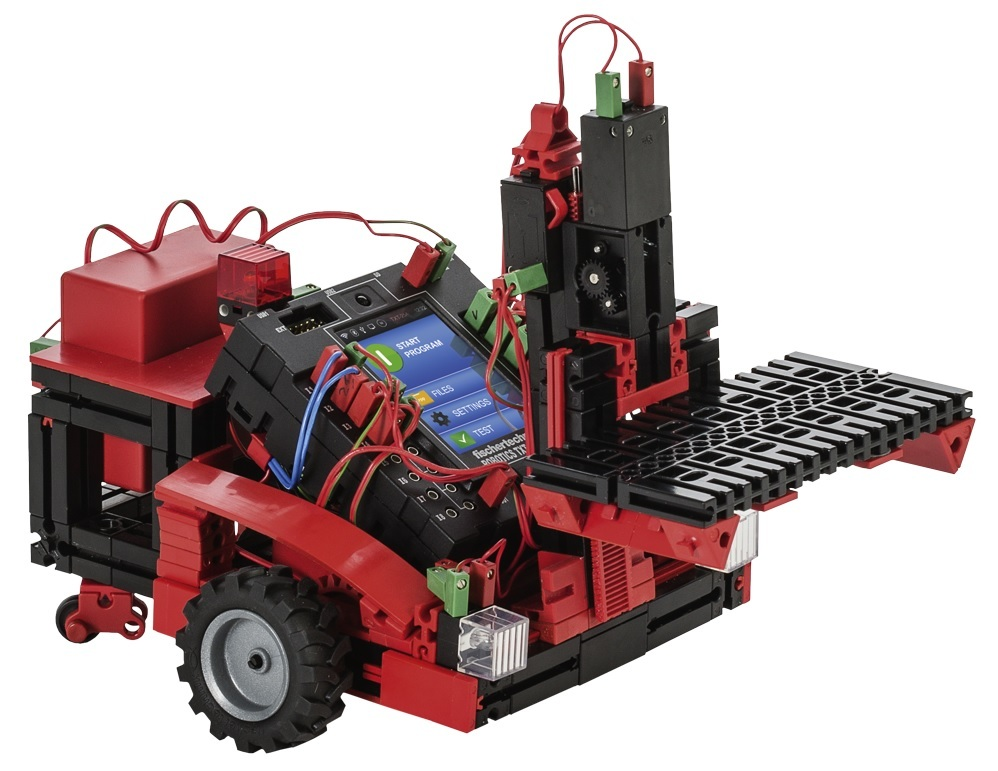
\includegraphics[width=250px]{images/fischertechnik_ROBO-TX-Explorer_02.jpg}
	\caption[Fischertechnik -- ROBO TX Explorer]{Fischertechnik -- ROBO TX Explorer\protect\footnotemark}
	\label{fig:fischertechnik_ROBO-TX-Explorer}
\end{figure}

\footnotetext{Zdroj: \url{http://www.helago-cz.cz/eshop-519143-workstation-robo-tx-training-lab-tx-explorer-146560.html}}

Existuje i mnoho podobných stavebnic~\cite{intorobotics_BestAlternativesToLegoMindstormsKits}. 
Například \fischerT prodává podobné robotické sety jako \lego{~}\cite{fischertechnik_ROBOTICS}. 

Uživateli nabízí rozsáhlejší pohled do elektroniky a~fungování jednotlivých modulů. 
Umožňuje také relativně snadno přidat vlastní moduly.
Zároveň má jednoduché grafické programovací prostředí podobně jako \lego. 
\FischerT{ }ovšem není tak rozšířen jako \legoM, protože ačkoliv nabízí v~některých ohledech více funkcí, zároveň klade větší nároky na uživatele, je podstatně dražší (základní set~\cite{fischertechnik_HelagoEshop_ROBOTICS-TXT-COMPETITION-SET} stojí cca dvakrát tolik co \legoEV{ Základní souprava}~\cite{lego_eduxeEshop_CoreSet}) a~nemá takový věhlas a~značku.

% figure + footnote -> minipage 
%src: http://www.tex.ac.uk/FAQ-ftncapt.html
% \begin{figure}[h]
% \begin{minipage}{\textwidth}
%  	\centering
% 	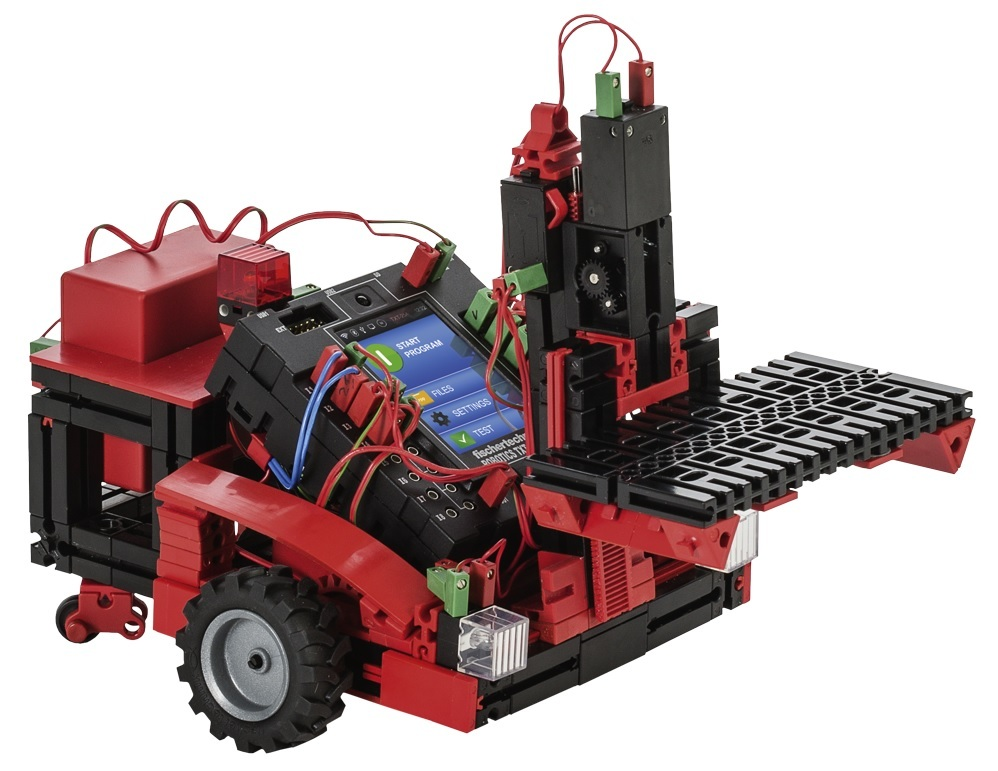
\includegraphics[width=300px]{images/fischertechnik_ROBO-TX-Explorer_02.jpg}
% 	\caption[Fischertechnik - ROBO TX Explorer]{Fischertechnik - ROBO TX Explorer \footnote{Zdroj: \url{http://www.helago-cz.cz/eshop-519143-workstation-robo-tx-training-lab-tx-explorer-146560.html}}
% \end{minipage}
% \end{figure}

% figure + footnote -> afterpage
% src: http://tex.stackexchange.com/questions/10181/using-footnote-in-a-figures-caption
%\afterpage{
%	\begin{figure}[h]
%	 	\centering
%		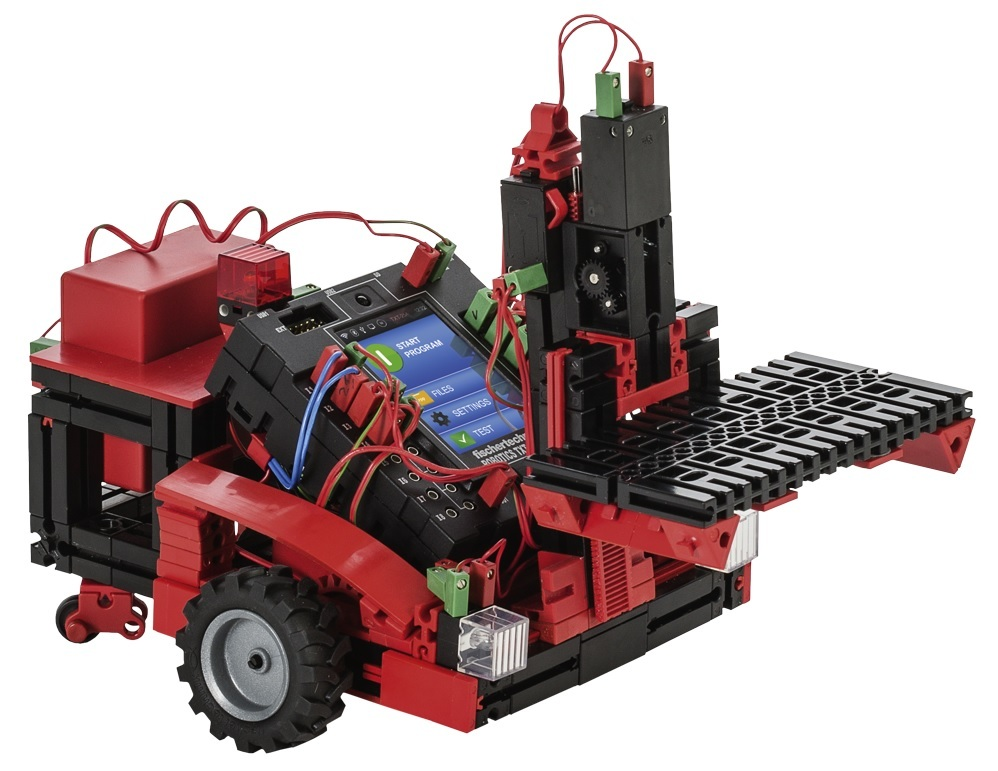
\includegraphics[width=300px]{images/fischertechnik_ROBO-TX-Explorer_02.jpg}
%			\caption[Fischertechnik - ROBO TX Explorer]{Fischertechnik - ROBO TX Explorer \footnotemark}
%		\label{fig:fischertechnik_ROBO-TX-Explorer}
%	\end{figure}
%	\footnotetext{Zdroj: \url{http://www.helago-cz.cz/eshop-519143-workstation-robo-tx-training-lab-tx-explorer-146560.html}}
%}

\begin{figure}[h]
	\centering
	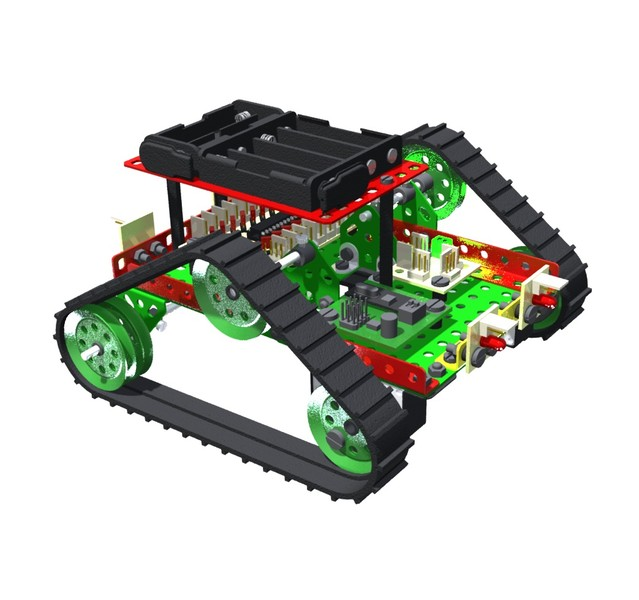
\includegraphics[width=235px]{images/MERKUR_Pasovy-podvozek-01_ATMEL+RC.jpg}
	\caption[MERKUR -- Pásový podvozek 01 -- ATMEL + RC]{MERKUR -- Pásový podvozek 01 -- ATMEL + RC\protect\footnotemark}
	\label{fig:MERKUR_Pasovy-podvozek-01_ATMEL+RC}
\end{figure}

\footnotetext{Zdroj: \url{http://www.merkurtoys.cz/vyrobky/pasovy-podvozek-merkur-s-elektronikou-rc}} 

Další zajímavou stavebnicí jsou Robotické sety od \merkur{u}~\cite{merkur_roboticsSetsEshop}. 
Nabídka jednotlivých setů je relativně široká a~v~porovnání s~\legoM{ }nebo \fischerT{ }nabízí ještě bližší kontakt s~elektronikou a~samotným hardwarem. 
Jako řídicí mikrokontroléry můžete využít PIC nebo megaAVR od firmy Microchip. 

Vzhledem k~použitým procesorům je možné tyto stroje programovat v~C/C++, PICAXE BASIC nebo i~v~grafickém prostředí~\cite{picaxeCz_BlocklyForPICAXE}. 
Robotické stavebnice od Merkuru mají podobné \uv{problémy} jako \fischerT. 
Kladou na uživatele větší nároky, nemají tak zvučnou značku, mají omezenější základní sadu senzorů a~neumožňují tak rychlou stavbu fungujícího robota.

Na závěr lze zmínit výukové roboty, kteří jsou primárně, na rozdíl od robotických stavebnic, zaměřeny na velmi úzkou oblast činností (jízda po čáře, plnění jednoduchých sekvenčních úkolů, \dots). 
Tyto roboty jsou zajímavé z~pohledu ceny, ale i~jednoduššího využití ve výuce (žáci nemusí sestavovat konstrukci a hardware je plně připraven k~používání). 

Naopak již neumožňují rozvoj kreativity studentů při stavbě a přizpůsobení robota pro různé soutěže (většinou je lze využívat jen v~jedné soutěžní kategorii).  
Mezi takovéto roboty patří například Pololu~3pi~\cite{robotPololu3pi} (primárně určen pro jízdu po čáře -- zvládá jezdit až~1~m/s) nebo Edison~\cite{robotEdison} (umí sledovat čáru, lze jej programovat graficky i~v~Pythonu, má různé senzory, je možné jej kombinovat s~\lego{ }kostkami). 

Tyto roboty ovšem neumožňují takový rozsah činností jako \legoM.

\begin{figure}[h]
	\begin{minipage}[b]{.5\textwidth}
		\centering
		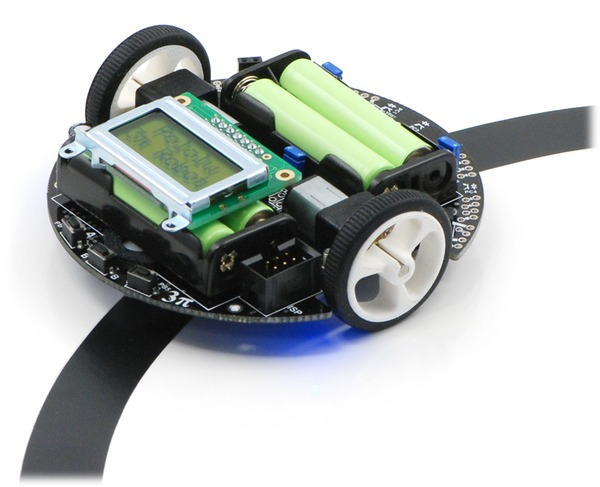
\includegraphics[width=\textwidth]{images/pololu-3pi-robot-8-on-line.jpg}
		\caption[Robot Pololu 3pi]{Robot Pololu 3pi\protect\footnotemark}
		\label{fig:pololu-3pi-robot-8-on-line}
	\end{minipage}
	\hfill
	\begin{minipage}[b]{.5\textwidth}
		\centering
		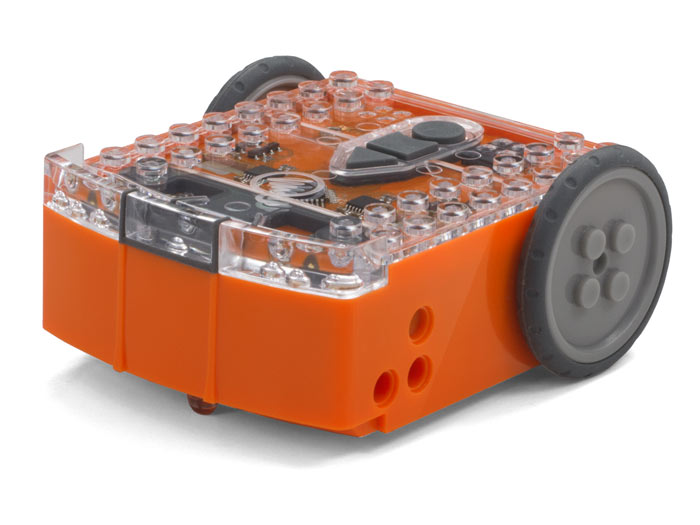
\includegraphics[width=\textwidth]{images/Edison-Educational-robot.jpg}
		\caption[Robot Edison]{Robot Edison\protect\footnotemark}
		\label{fig:Edison-Educational-robot}
	\end{minipage}
\end{figure}

% two footnote/footnotemark in minipage - problem with index
% solution: http://tex.stackexchange.com/a/43694

\addtocounter{footnote}{-1} % footnote_cnt -= 1
\footnotetext{Zdroj: \url{https://www.pololu.com/product/975}}
\stepcounter{footnote}
\footnotetext{Zdroj: \url{https://meetedison.com/meet-edison-v2-0/}}


% putting two images beside each other
% source: http://tex.stackexchange.com/a/148445

%\begin{figure}[!tbp]
%	\begin{subfigure}[b]{.5\textwidth}
%		\centering
%		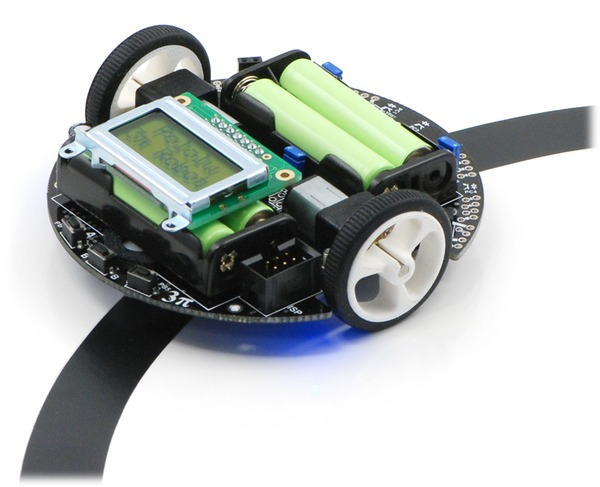
\includegraphics[width=\textwidth]{images/pololu-3pi-robot-8-on-line.jpg}
%		\caption[Robot Pololu 3pi]{Robot Pololu 3pi\protect\footnotemark}
%		\label{fig:pololu-3pi-robot-8-on-line}
%	\end{subfigure}
%	\hfill
%	\begin{subfigure}[b]{.5\textwidth}
%		\centering
%		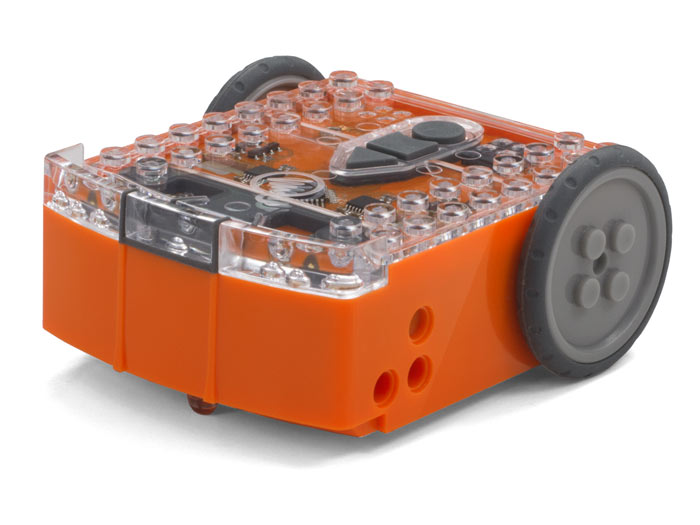
\includegraphics[width=\textwidth]{images/Edison-Educational-robot.jpg}
%		\caption[Robot Edison]{Robot Edison\protect\footnotemark}
%		\label{fig:Edison-Educational-robot}
%	\end{subfigure}
%	\caption{Roboti se zaměřením na velmi úzkou oblast činnost}
%\end{figure}
%
%\footnotetext{Zdroj: \url{https://www.pololu.com/product/975}} 
%\footnotetext{Zdroj: \url{https://meetedison.com/meet-edison-v2-0/}} 

\section{Motivace autora}

Již čtvrtým rokem vedu robotický kroužek na své bývalé střední škole SPŠ a VOŠ Brno, Sokolská a~zároveň organizuji tábory a~další vzdělávací akce v~oblasti techniky a~robotiky na pobočce Robotárna, Dům děti a~mládeže Brno, Helceletova.
Už na střední škole jsem se v~rámci těchto dvou organizací účastnil různých soutěží, jako například Robotický den v~Praze, Mikrokontroléry letí na FEKT VUT Brno nebo Středoškolská odborná činnost (obory strojírenství a~elektrotechnika). 
Z~některých soutěží jsem si dovezl cenná umístění, ale~i~mnoho zkušeností, inspirace a~podnětů na přemýšlení.


Za dobu, kterou se věnuji programování mikrokontrolérů a~robotice, jsem již narazil na mnoho překážek a~problémů, které bylo třeba překonat. 
%si už mnohokrát prošel trnitou cestou 
Tyto překážky jsou ovšem výrazně náročnější pro studenty, kteří v~těchto oblastech teprve začínají a~seznamují se s~nimi. 

Často může nastat i~situace, kdy je student se zájmem o~robotiku odrazen její počáteční složitostí.

Přitom by z~něj mohl být v~budoucnu perfektní programátor. 
Jen mu zrovna tenhle mikrokontrolér nejde naprogramovat nebo mu koupený H-můstek nechce roztočit motor.

Proto se svým studentům vždy snažím nachystat co nejlepší prostředí pro začátky s~robotikou. 

Již jsem zkoušel různé platformy (například využít k~výuce robota Pololu~3pi) i~způsoby výuky (kombinace elektroniky, programování na PC a~programování mikrokontrolérů), ale~bohužel vždy jsem se dostal do stejné situace. 

Ačkoliv mi studenti chodili již rok do robotického kroužku, pořád je dělily minimálně dva roky od schopnosti postavit a~naprogramovat složitějšího robota (s~tím, že by použili předpřipravenou elektroniku, ale rozuměli tomu, co je jak zapojeno + uměli použít dostupné knihovny a~naprogramovat si chování svého robota).

Nedávno jsme ale do kroužku zakoupili \legoEV{}. 
Stavebnici, která mi měla umožnit postavit robota za den. 
Prakticky stavebnice snů. No není to nádherná představa?
A~opravdu tomu tak bylo. Robota jezdícího po čáře jsme s~manuálem zvládli poskládat a~zprovoznit za den. 
Studenti nemuseli studovat a~řešit zapojení jednotlivých komponentů do řídicí elektroniky. 

Nebylo třeba trávit mnoho času vysvětlováním způsobu programování 8bitových mikrokontrolérů (omezení paměti a~výkonu, menší datové typy -- \verb|uint_8t|, komunikace po sériové lince, \dots).

Jen si poskládali z~\lega{ }hardware, pomocí kabelů (které nelze otočit ani zapojit špatně a~tím něco zničit) spojili jednotlivé moduly. 

A~v~grafickém prostředí si poskládali svůj program.

Pak jsme se ale začali soustředit na zlepšování softwaru i~hardwaru tak, abychom využili stavebnici na 100~procent, a~v~ten moment jsme narazili.

Dokud jsme si s~EV3 jen \uv{hráli} a~nesoustředili se primárně na výkon a~spolehlivost, bylo vše v~pořádku. 
Jakmile jsme ale chtěli mít regulační smyčku PID~regulace pro robota na sledování černé čáry s~periodou 10~ms, zjistili jsme, že to nejde (a~to máme v~EV3 \brick{\it u} 300~MHz~ARM). Přitom díky předešlým zkušenostem s~8bitovými mikrokontroléry Atmel~AVR jsme věděli, že by to neměl být problém.


To samé platí o~grafickém vývojovém prostředí dodávaném s~\EVthree. Dokud máte na obrazovce několik programových bloků, vše funguje bez problémů. 
Když se však program rozroste na několik obrazovek a~samostatných modulů, velmi rychle ztrácíte přehlednost a~efektivitu programování.
Zároveň vám již moc nepomohou ladicí nástroje, které jsou součástí prostředí, protože při jednoduchém programu je lze relativně dobře využít, ale při rozsáhlejších programech již nejsou k~dispozici nebo je jejich použití velmi komplikované. 


Proto jsme začali hledat alternativní platformy, které by odstraňovaly zmíněné problémy, což vyústilo v~tuto práci.   


  
  \chapter{Historie \legoM}

Historie firmy \lego{ }je velmi dlouhá a~sahá až do roku 1932~\cite{lego_GroupHistory1930s}. 
V období, kdy se počítače stávají standardní součástí domácnosti, se dostávají í do \lego{} a tím roku 1998 vzniká  \legoM{}~\cite{lego_mindstormsHistory}.
% * <kuba.streit@gmail.com> 2017-05-07T14:53:32.539Z:
% 
% Postupně čtu a myslím si:
% LEGO 1932 - super, Mindstorms prakticky to samé? Zajímavé, to bych nečekal. To samé = 1998 - what?
% Spíš bych to asi zkusil přeformulovat tak nějak, jako že v období, kdy se počítače stávají standardní součástí domácnosti, dostávají se i do Lega a tím vzniká Mindstorms.
% 
% ^ <paral.jarek@gmail.com> 2017-05-07T19:10:12.410Z:
%
% Předělám.
%
% ^ <paral.jarek@gmail.com> 2017-05-07T21:57:01.485Z:
%
% Hotovo.
%
% ^.

% TODO: kapitola LEGO TECHNIC

\section{\legoM{ }RCX}

První verze byla označena jako \legoM{ }RCX\footnote{RCX = Robotic Command eXplorers} Intelligent Brick and Robotics Invention System a~obsahovala 8bitový mikrokontrolér Hitachi H8/3292~\cite{hitachi_microcontrolerH8series} s~procesorem H8/300 taktovaným na 16~MHz a~s~32~KB~RAM~\cite{legoMindstormsRCX_Manual}.

\begin{figure}[h]
	\centering
	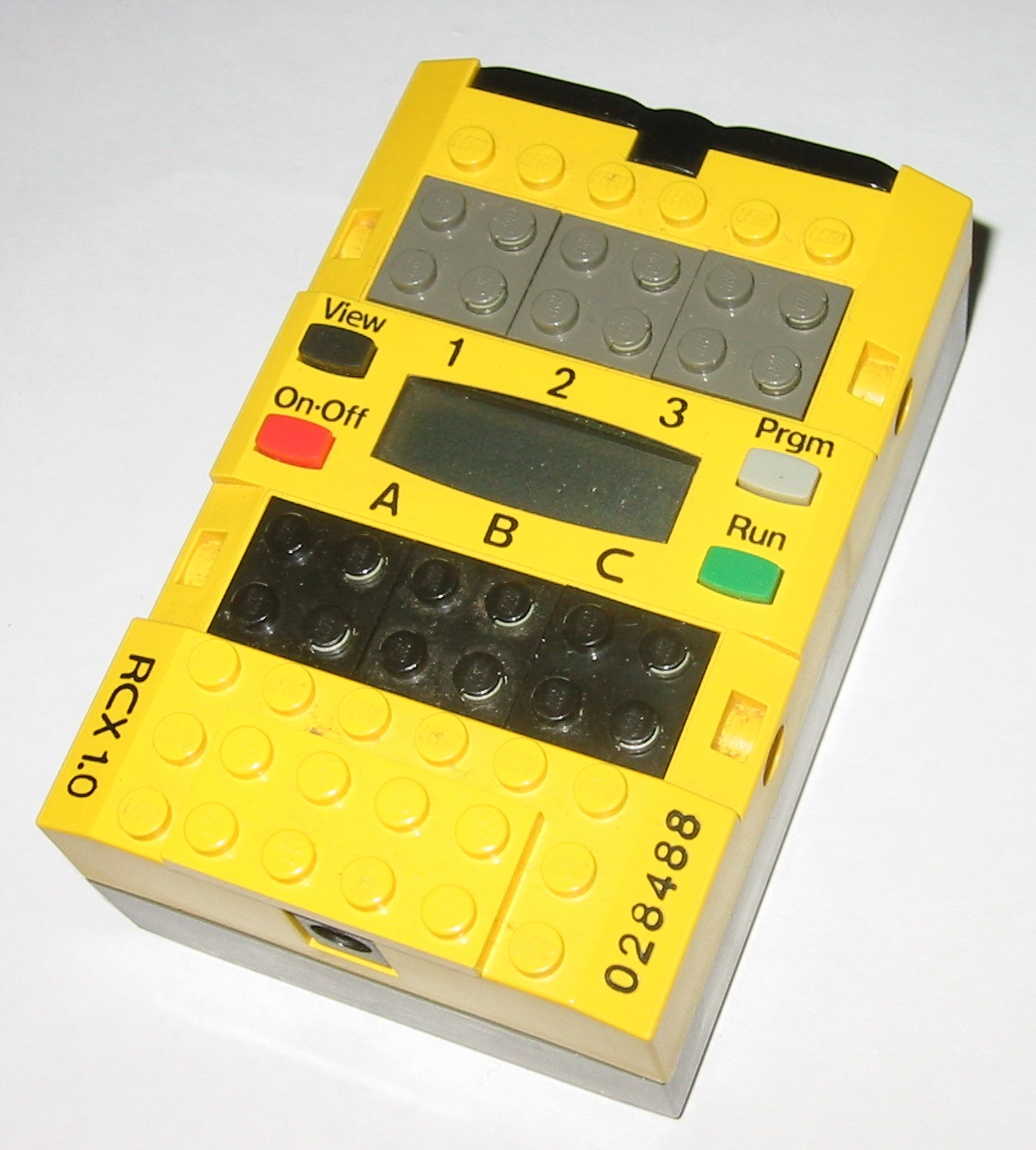
\includegraphics[width=250px]{images/lego-mindstorms-rcx_wikipedia.jpg}
	\caption[\legoM{ }RCX]{\legoM{ }RCX\protect\footnotemark}
	\label{fig:lego-mindstorms-rcx-wikipedia}
\end{figure}

\footnotetext{Zdroj: \url{https://en.wikipedia.org/wiki/Lego_Mindstorms}} 

Oficiálně bylo možné stavebnici programovat ve dvou prostředích. První prostředí ROBOLAB, založené na programu \labview{ }od firmy \NI, bylo pro výukové účely (do škol) a~bylo součástí výukového setu. 
Běžní zákazníci (lidé, kteří si kupovali stavebnici domů) měli k~dispozici RCX Code, které bylo jednodušší na obsluhu a používání, ale nemělo tak rozsáhlé možnosti programování. 
Zároveň vznikla i~vývojová prostředí třetích stran, která umožňovala programování v~mnoha běžně používaných jazycích (C++, Java,~\dots).

Již v~prvním roce prodeje stavebnice vznikla soutěž {\it FIRST} LEGO League (FLL)\footnote{{\it FIRST} = For Inspiration and Recognition of Science and Technology}. 
Cílem soutěže je povzbudit a~motivovat k~navrhování, stavění a`programování vlastních inteligentních systémů~\cite{lego_FLL-about}. 
Jednotlivá kola probíhají po celém světě a~lze postoupit až do celosvětového finále. % TODO: FLL - ověřit možnost postupu do celosvětového finále
Účastníci musí být ve věku od 10 do 16 let. 

\section{\legoM{ }NXT}

Následující verzi vydalo \lego{ }v roce 2006~\cite{lego_mindstormsHistory}. 
Byl kompletně změněn způsob připojování jednotlivých modulů. 
Moduly se již nepřipojují pomocí speciálních \lego{ }kostek, ale využívají upravený konektor RJ-12 % TODO: upravený konektor -> méně běžnou variantu konektoru RJ-12
(kolík sloužící pro správné zapojení konektoru je oproti běžné telefonní RJ-12 umístěn mimo střed~\cite{legoMindstorms_rj12-connector}). % -- na pravou stranu z pohledu od kabelu 

\begin{figure}[h]
	\centering
	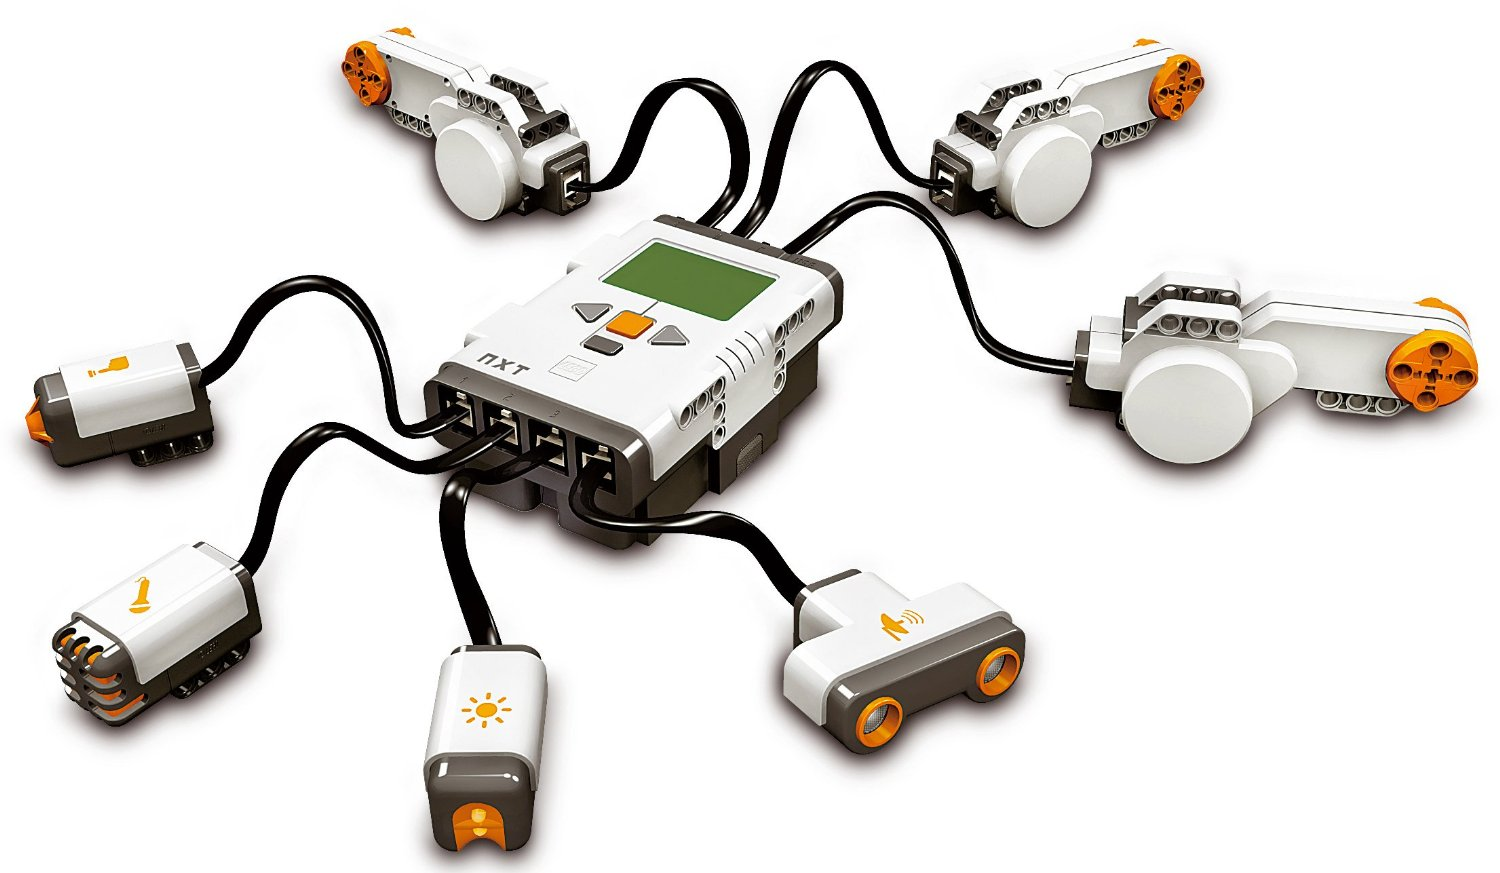
\includegraphics[width=\textwidth]{images/lego-mindstorms-nxt_with-modules.jpg}
	\caption[\legoNXT{ }s komponenty, které lze používat]{\legoNXT{ }s komponenty, které lze používat\protect\footnotemark}
	\label{fig:lego-mindstorms-nxt_with-modules}
\end{figure}

Řídicí kostka (dále jen \brick{}) % TODO: formátování speciálních výrazů

se již neprogramuje přes infraport, ale využívá se standardní USB kabel, případně integrovaný Bluetooth~\cite{legoMindstormsNXT_hardware}.

Po hardwarové stránce došlo ke značnému posunu. Původní 8bitový mikrokontrolér byl nahrazen 32bitovým ARM mikrokontrolérem % TODO: mikrokontrolér/mikroprocesor/procesor

AT91SAM7S256 (256~KB~FLASH, 64~KB~RAM, 48~MHz) a~k~němu byl přidán 8bitový ko-procesor ATmega48 (4~KB~FLASH, 512~Byte~RAM, 8~MHz). 
Oba tyto procesory dodávala firma Atmel (nyní již Microchip)~\cite{legoMindstormsNXT_hardware}.

\footnotetext{Zdroj: \url{http://www.itnetwork.cz/java/lego-nxt/seznameni-s-nxj-pro-lego-nxt}} 

\brick{ }lze programovat pomocí vývojového prostředí NXT-G\footnote{NXT-G = NXT Graphic - grafické} (viz obrázek \ref{fig:lego-mindstorms-nxt-g}), které \lego{ }vyvinulo opět ve spolupráci s~\NI{~}\cite{legoMindstormsNXT_NXT-G}. 
Zároveň \NI{ }dodává toolbox do \labview{}, ve kterém lze \brick{ }také programovat. 

\legoNXT{ }má ovšem bohatou nabídku alternativních programovacích prostředí, která lze využít k~vytváření kódu pro \brick. 
Některá fungovala již na RCX a~byla upravena i~pro NXT. 
Jako příklad mohu uvést jedno z~nejpoužívanějších prostředí BricxCC\footnote{BricxCC = Bricx Command Center} s~jazykem NXC\footnote{NCX = Not eXactly C}. 
NCX je vysokoúrovňový open-source jazyk podobný C~\cite{legoWikipediaNXT_NXC}.

\begin{figure}[h]
	\centering
	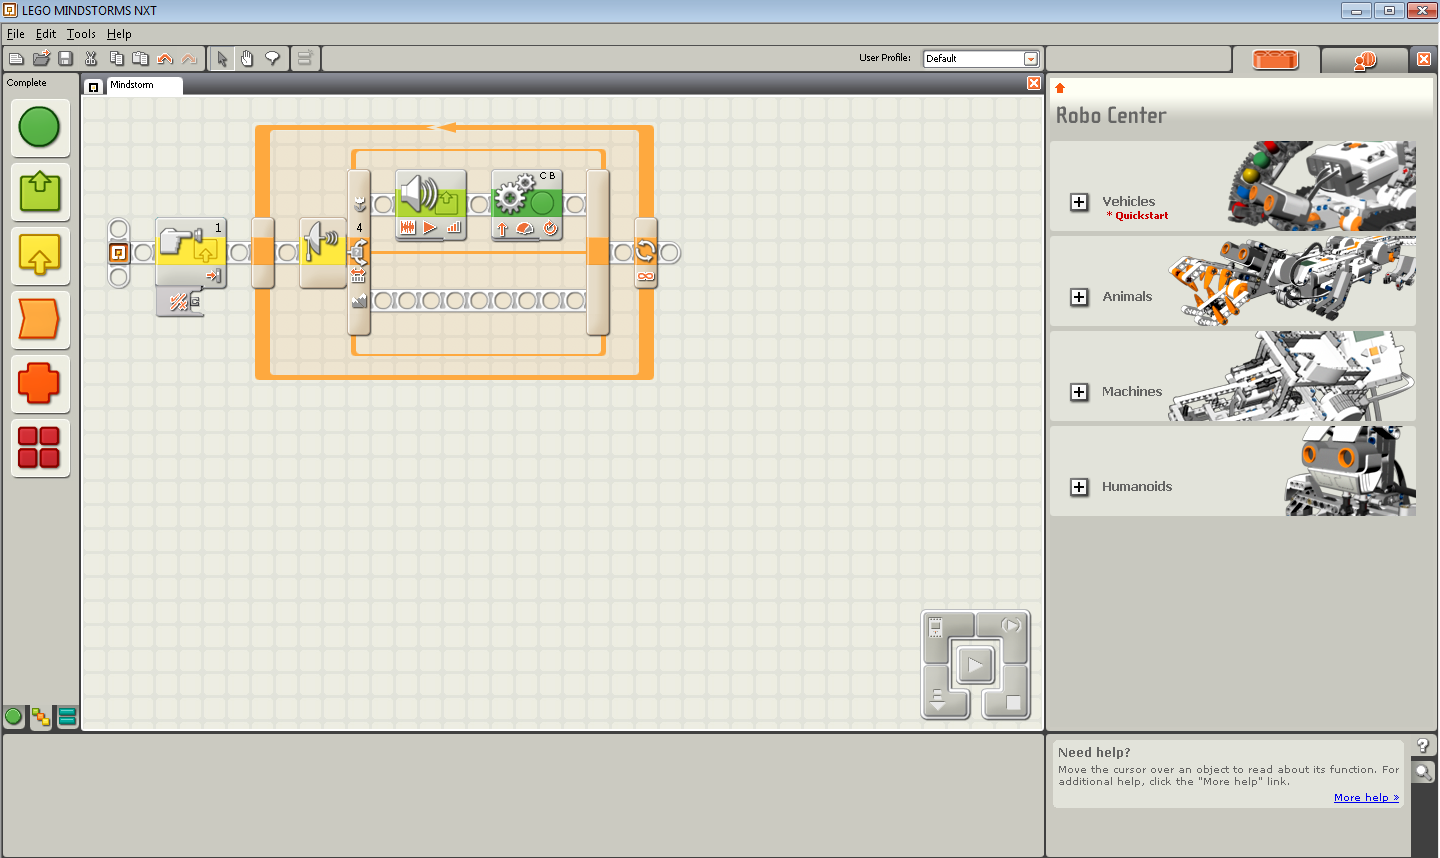
\includegraphics[width=\textwidth]{images/lego-mindstorms-nxt-g.png}
	\caption[\legoNXT{-G}]{\legoNXT{-G}\protect\footnotemark}
	\label{fig:lego-mindstorms-nxt-g}
\end{figure}

\footnotetext{Zdroj: \url{http://lukedainton-robots.blogspot.cz/2012/07/control-systems-shooterbot-nxt-g.html}} 
Existují ale i~komerční varianty. 
Například ROBOTC~\cite{legoProgramingPlatform_ROBOTC} je univerzální programovací prostředí a~jazyk umožňující programovat větší množství hardwaru (od \legoM{ }RCX, NXT, EV3 až po Arduino nebo PIC). 
Jak již název napovídá, ROBOTC je založen na jazyku C (ANSI-C).
Uživatel ovšem může přecházet mezi grafickou a~textovou formou programování, což může být pro začátečníky velmi vhodné.
Také má možnost vybrat si úroveň abstrakce, na jaké bude v~textovém módu pracovat.  

ROBOTC je velmi zajímavé prostředí. Bohužel nikdy nebyla vydána objektová varianta, s~kterou by mohlo být programování ještě jednodušší. 
Zároveň se jedná o~placený produkt a~jednotlivé licence~\cite{legoProgramingPlatform_ROBOTC-price} tvoří přibližně čtvrtinu současné ceny základní sady stavebnice \legoEV{~}\cite{lego_eduxeEshop_CoreSet}, což už není nezanedbatelná částka.

Pro NXT existuje celá řada dalších platforem a~jazyků (Javy, C\#, Lua, Ada, Python~\cite{legoMindstormsNXT_Programming}), které lze použít. 
Jelikož je ale tato práce zaměřena na \legoEV{ }, nebudou tyto platformy dále řešeny. 

\section{\legoM{ }EV3}

Aktuálně nejnovější verzí stavebnice \legoM{ }je verze EV3, která byla vydána v~roce 2013~\cite{lego_mindstormsHistory}. 
Proběhlo u~ní mnoho inovací a~změn, i~tak ale byla zachována velmi dobrá kompatibilita s~verzí NXT~\cite{legoRobotSquare_EV3-and-NXT-compatibility}.

EV3 přináší zásadní změnu procesoru. 
Jedná se o~32-bitový~ARM (ARM9), tentokrát ale od firmy Texas Instrument, s~označením AM1808 (16~MB~FLASH, 64~MB~RAM, 300~MHz)~\cite{legoMindstormsEV3_fw-dev-kit}. 
Kvůli správě paměti již musí tento procesor používat operační systém. % TODO: doplnit info o správě paměti na ARM9 
\lego{ }pro EV3 vytvořilo upravenou verzi Linuxu. 

\begin{figure}[h]
	\centering
	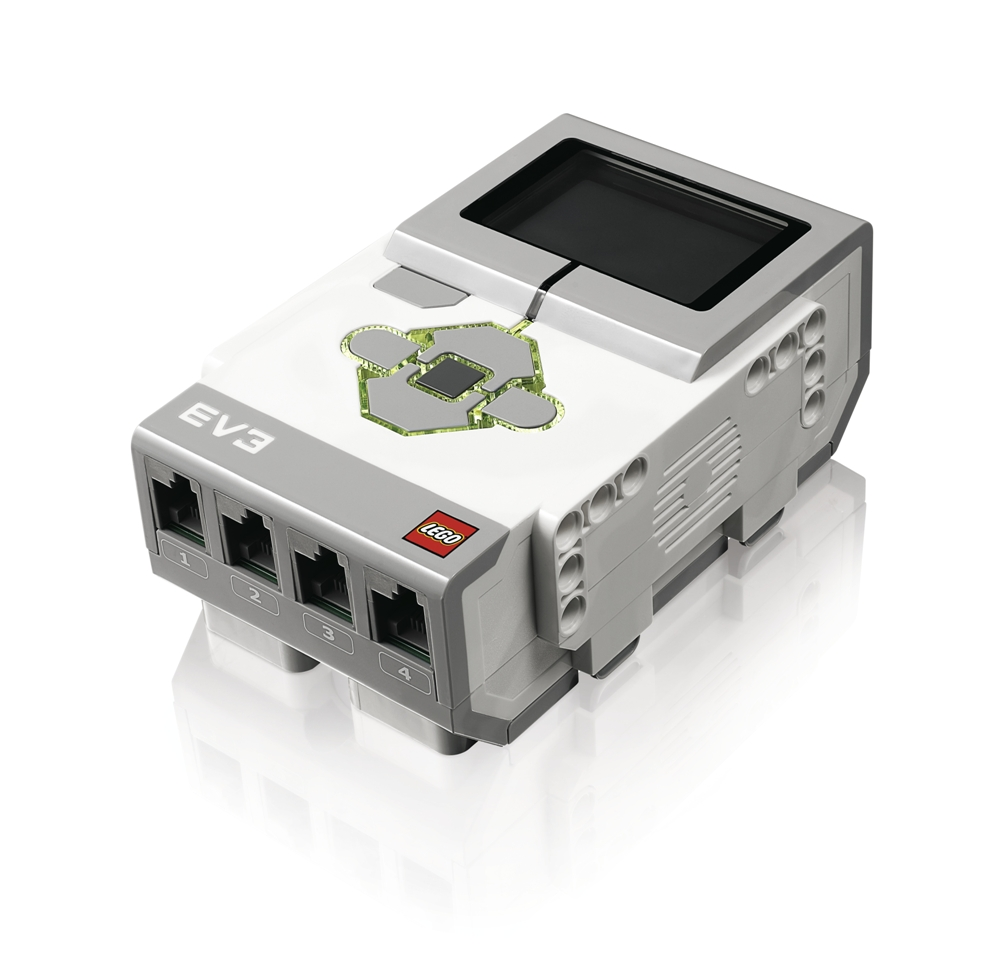
\includegraphics[width=330px]{images/lego-mindstorms-ev3_brick.jpg}
	\caption[\legoEV{ Brick}]{\legoEV{ \brick}\protect\footnotemark}
	\label{fig:lego-mindstorms-ev3_brick}
\end{figure}

\footnotetext{Zdroj: \url{http://hackeducation.com/2015/04/10/mindstorms}} 

Nová verze obsahuje také čtečku Micro SD karet, USB host interface a~jeden výstupní port pro motory navíc (celkem 4~porty, NXT jen 3~porty) \cite{legoBotBench_comparing-EV3-and-NXT}. 

Slot na SD karty umožňuje rozšířit paměť pro programy, ale lze jej hlavně využít pro spouštění alternativních operačních systémů. 

Díky USB host interface lze k~EV3 připojovat různé periferie, pro které je v~systému a~vývojovém prostředí připravená obsluha.
Lze tak připojit Wifi modul nebo klávesnici. 
% * <kuba.streit@gmail.com> 2017-05-07T15:03:27.550Z:
% 
% Musí to umět systém, vývojové prostředí bych tu nezmiňoval. 
% Navíc z toho, co jsme zkoušeli, jediný prostředí, který umí víc než Wifi, je ev3dev.
% 
% ^ <paral.jarek@gmail.com> 2017-05-07T18:50:35.270Z:
%
% JJ to musím přeformulovat:  "Díky USB host interface lze k~EV3 připojovat různé periferie, pro které je v~systému a~vývojovém prostředí připravená obsluha.
% Lze tak připojit Wifi modul, klávesnici nebo myš. "
%
% ^ <paral.jarek@gmail.com> 2017-05-08T13:29:14.648Z:
%
% Ponecháno.
%
% ^.
Zároveň můžete přes USB kabel spojit až čtyři EV3 \brick{\it y} a~ovládat je jedním programem (z~jednoho hlavního \brick{\it u}).

\begin{figure}[h]
	\centering
	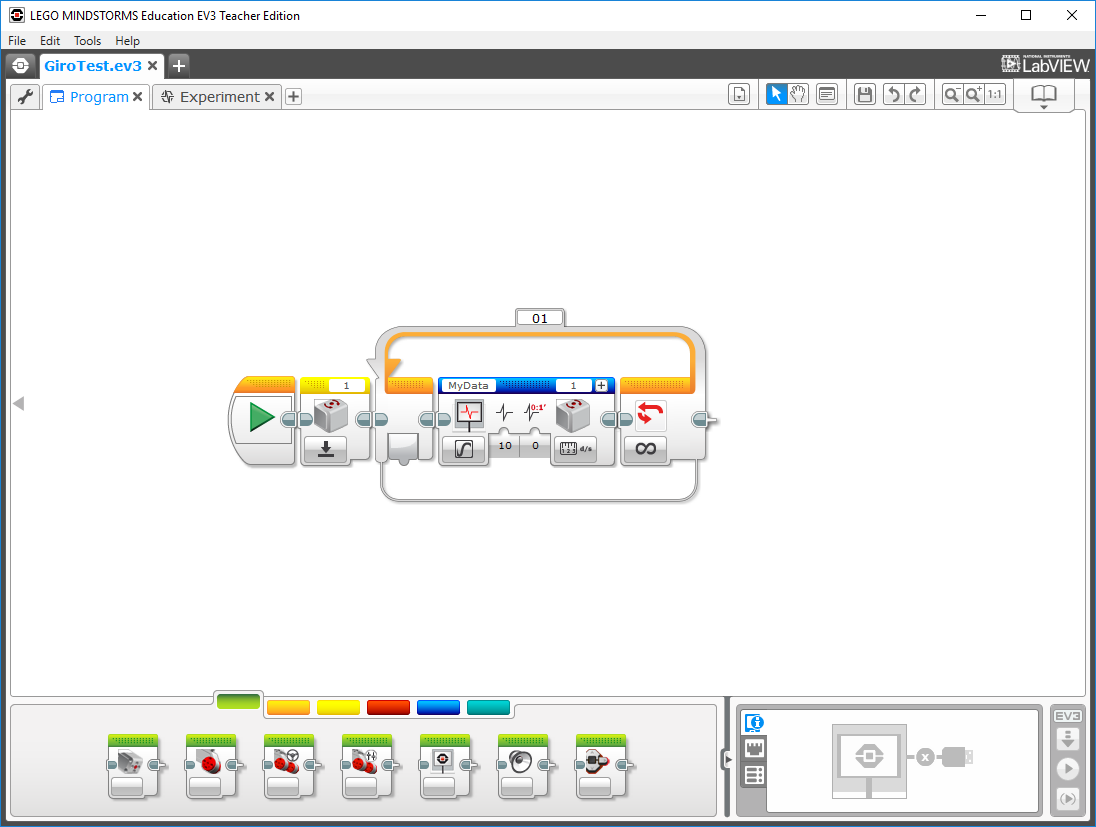
\includegraphics[width=\textwidth]{images/lego-mindstorms-ev3_dev-soft.png}
	\caption[\legoM{ }Education EV3 Software -- vývojové prostředí]{\legoM{ }Education EV3 Software -- vývojové prostředí}
	\label{fig:lego-mindstorms-ev3_dev-soft}
\end{figure}

Programovací prostředí pro EV3 je znovu postaveno na \labview{ }a~ačkoliv se design v~porovnání s~prostředím pro NXT výrazně změnil (můžete porovnat obrázky \ref{fig:lego-mindstorms-nxt-g} a~\ref{fig:lego-mindstorms-ev3_dev-soft}), neměli by mít uživatelé NXT s~přechodem problém. 
Nové prostředí zvládne naprogramovat jak EV3, tak NXT \brick{}.

V~rámci alternativních platforem máme opět velký výběr \cite{legoMindstormsWikipedia_programming-languages}. 
Vhledem k~nutnosti používání operačního systému je většinou pro dané prostředí potřeba nahrát konkrétní systém na SD kartu a spustit \brick{ }s~touto kartou.

Jednotlivé alternativní platformy budou podrobněji probrány v~následující kapitole.

  
  \chapter{Testování}
\label{testing}

Cílem testování v~této kapitole je zjistit výkonnost jednotlivých platforem a~porovnat je vůči sobě. 
Testy jsou zaměřeny primárně na měření časů průběhu hlavní smyčky při určitých činnostech tak, aby bylo možné srovnat výkonnost a~stabilitu jednotlivých platforem. 
Stabilitou je v~tomto případě myšlen rozdíl mezi průměrným a~maximálním naměřeným časem průchodu smyčky v~rámci opakovaných měření a~jednotlivých průchodů.

Při předchozí práci s~\EVthree{ } se systémem \evThreeDev (viz kapitola~\ref{lego-ev3dev}), že minimální perioda hlavní smyčky s~pár příkazy na vyčtení dat ze senzoru a~následného nastavení motorů dle těchto hodnot (klasický program na jízdu po čáře) není kratší než 10~ms. 
Vzhledem k~výkonu procesoru (32bitový ARM na 300~MHz) v~\EVthree{ }je tento čas velmi zarážející. 

O~to větší překvapení nastalo, když jsem srovnával průměrnou periodu s~maximální. Ukázalo se, že ačkoliv je průměrná perioda přibližně 20~ms, maximální perioda může dosahovat až~100~ms. 
Takto velký rozptyl je pro potřeby regulace velmi problematický. 
Ve většině případů je potřeba mít konstantní čas průchodu hlavní smyčkou, aby rozdíl v~časech periody neovlivňoval měření a~následné řízení. 

Pokud bude nutné zajistit stabilní periodu, je třeba softwarově zpomalit průběh hlavní smyčky na maximální naměřený čas. 
Jedině tak lze zajistit konstantní periodu. 
Když by se použil tento postup, dostali bychom se na frekvenci 10~Hz, což je z~pohledu regulace již velmi nepříznivá hodnota.

Tyto testy byly provedeny na velmi jednoduchém programu. 
V~případě rozsáhlejších projektů, kde by se pracovalo s~více vlákny a~periferiemi, mohou být výsledky ještě horší.

Proto jsem chtěl provést testování s~ekvivalentními programy na jednotlivých platformách a~zjistit, jestli tyto neduhy některá z~nich neodstraňuje a~za jakých situací k~podobným problémům dochází.

\section{Forma testování}

Na počátku jsem zvažoval dvě formy testování. První počítala s~rozsáhlejší metodikou, v~rámci které bych testoval různé funkce \EVthree{}~\brick{{\it u}} a~zjišťoval, kde mohou být nejproblémovější místa z~pohledu výkonu. \\

V~rámci testů jsem se chtěl zaměřit na několik oblastí: % a jejich kombinace.

\begin{itemize}
	\item matematické operace
	\item čtení senzorů
	\item řízení motorů
\end{itemize}  

Tuto variantu jsem na počátku odložil, abych zkusil najít metodu jednoduší na implementaci a~replikaci na jiné platformy. Následně v~ní ale pokračuji v~další části kapitoly.

Druhá varianta měla zajistit co možná nejstejnoměrnější podmínky měření času tak, aby jej neovlivňovalo fungování jednotlivých platforem. 
Proto mělo být k~měření využito Arduino Uno a~velmi jednoduchý program  (příklad programu ve standardním prostředí pro \EVthree{ }na obrázku \ref{fig:LoopTimeLEDblinking-measuring}).
Program by jen blikal s~dvěma LED\footnote{LED = Light-Emitting Diode –- dioda emitující světlo} (zelenou a~červenou) umístěnými na přední straně pod ovládacími tlačítky na \EVbrick{{\it u}} a~čas svitu jednotlivých LED by měřilo Arduino.

%U jednotlivých platforem by se měřili časy průchodů hlavní smyčkou a z těchto naměřených dat by se vytvářeli histogramy pro následné vyhodnocení.

% Následně jsem se ale rozhodl pro jinou strategii testování. 
% Rozhodl jsem se ale pro jinou strategii testování. 

% Po čase jsem tuto strategii zavrhl. 

Jednalo by se totiž o~jeden z~nejlepších způsobů, jak demonstrovat problémy s~dobou trvání jednotlivých cyklů a~práci s~periferiemi. 
V~optimálním případě by totiž měla kombinací těchto dvou barevných LED vzniknout oranžová. 

Pokud by se tak nestalo, pozorovatel by měl hned optickou zpětnou vazbu a~zároveň lze jednoduše měřit časové prodlevy mezi spínáním a~vypínáním jednotlivých LED pomocí měřicí sestavy s~Arduinem.

\section{Měření pomocí LED}


\begin{figure}[h]
	\centering
	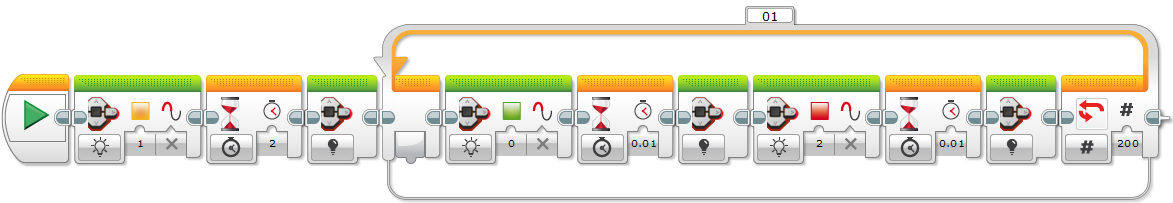
\includegraphics[width=\textwidth]{images/measuring-ev3-software_LoopTimeLEDblinking.png}
	\caption[Ukázka jednoduchého programu na blikání zelenou a~červenou LED]{Ukázka jednoduchého programu na blikání zelenou a~červenou LED}
	\label{fig:LoopTimeLEDblinking-measuring}
\end{figure}

Ukázkový program je připraven tak, že každá LED se vždy rozsvítí na 10~ms ($T~=~0.01~s~= 10~ms$), následně zhasne a~rozsvítí se druhá LED. 

Celkový čas jednoho průchodu cyklem trvá 20~ms ($T~=~T_{LED1}~+ T_{LED2}$) a~frekvence blikání by měla být 50~Hz ($f~=~\frac{1}{T}~= \frac{1}{0.02~s} =~50~Hz$). 
Což je frekvence, kterou již lidské oko nezaznamená (filmy mají standardní frekvenci obnovování snímku 24 až 30~Hz). % TODO: a běžné televizní vysílání má 50~Hz).
Celkový počet opakování hlavní smyčky je zvolen na 200. 
Blikání má tedy probíhat 4~sekundy ($t~=~T~\cdot~counter =~0.02~ms~\cdot~200~= 4~s$).

Pro měřicí sestavu byl vybrán fototranzistor BPX~81\footnote{\url{http://cz.rs-online.com/web/p/fototranzistory/6655255/}} (má velmi široké rozpětí vstupních vlnových délek -- zvládne viditelné i~infra světlo) s~Arduinem Uno (viz obrázek~\ref{fig:arduino-measuring-system}). \\

Tato kombinace mi přijde nejvhodnější z~několika důvodů: 

\begin{itemize}
	\item velmi rozšířený hardware (Arduino Uno)
	\item rychlé sestavení
	\item možnost snadného naprogramování
	\item jednoduchá duplikovatelnost (zopakování experimentu)
\end{itemize}  

Nejdůležitějším bodem pro tuto variantu byla jednoduchá duplikovatelnost, která umožňuje komukoliv provést stejná měření, ať už pro kontrolu v~této práci prezentovaných výsledků, nebo pro otestování jiné platformy a~porovnání s~naměřenými daty z~této práce.

\begin{figure}[h]
	\centering
	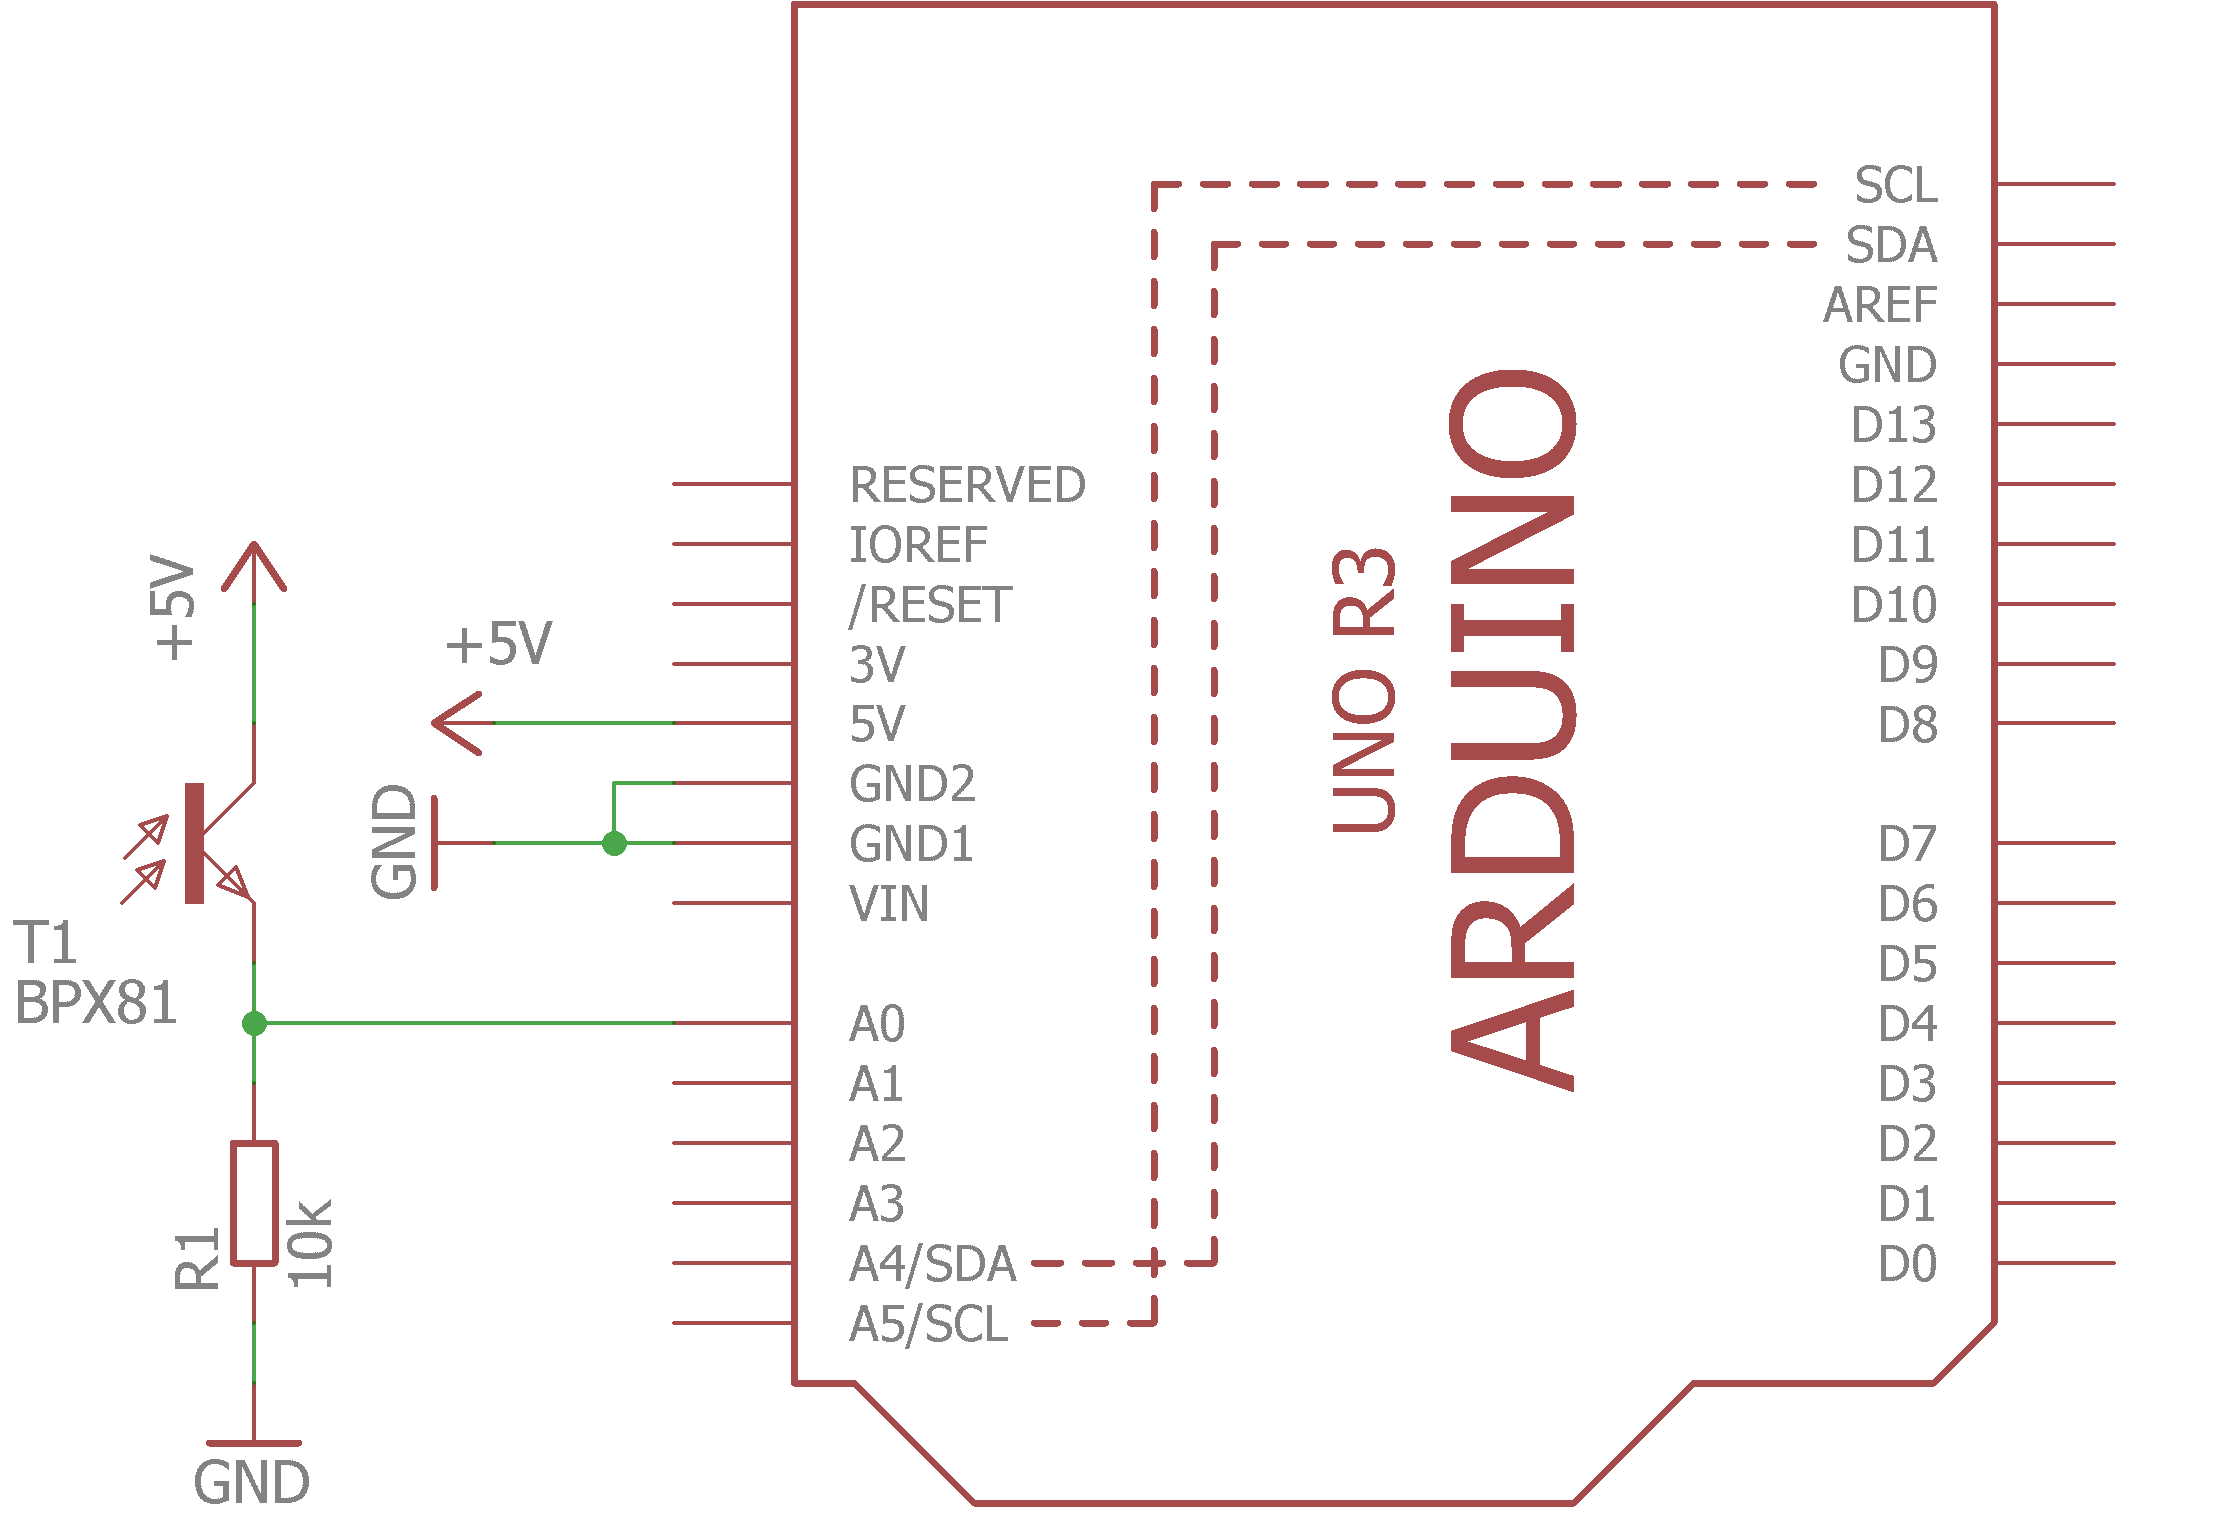
\includegraphics[width=250px]{images/measuring-arduino-system_schema.png}	
	\caption[Schéma zapojení měřicího systému]{Schéma zapojení měřicího systému}
	\label{fig:arduino-measuring-system}
\end{figure}

Jelikož se druhá varianta zdála vhodnější, otestoval jsem ji s~programem, prezentovaným výše, s~danou měřicí sestavou a~osciloskopem. 

\begin{figure}[h]
	\centering
	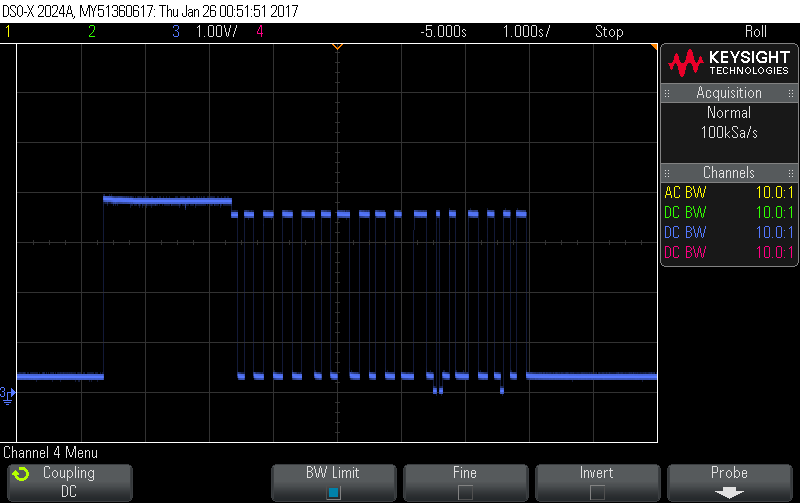
\includegraphics[width=350px]{images/measuring-oscilloscope_ev3-software_led-blinking_all.png}
	\caption[Záznam signálu z~osciloskopu po provedení zkušebního programu]{Záznam signálu z~osciloskopu po provedení zkušebního programu}
	\label{fig:measuring_lego-ev3_orig-soft_led-blinking_all}
\end{figure}

Výsledky byly velice překvapivé. Celkový počet pulzů červené LED (napětí na osciloskopu přibližně 3,7~V; pro zelenou 0,3~V; oranžová 3,9~V) byl 17 
(viz obrázek~\ref{fig:measuring_lego-ev3_orig-soft_led-blinking_all}). Přičemž dle programu mělo proběhnout 200~pulzů.  

Při detailním zkoumání se ukázalo, že LED nedokáží blikat na 50~Hz, ale mohou svůj stav měnit vždy s~frekvencí 20~Hz. 
Každých 50~ms docházelo ke kontrole stavových proměnných u~LED a~případné změně stavu (viz~obrázek~\ref{fig:measuring_lego-ev3_orig-soft_led-blinking_part1} -- jeden dílek odpovídá 100~ms a~1~V).

Toto chování lze například vysvětlit tak, že v~rámci operačního systému \EVbrick{\it u} je v~určité periodě (přibližně 50~ms) vyvoláno přerušení od časovače, které porovná stav proměnných a~registrů LED a~dle výsledku buď rozsvítí, nebo zhasne. 
Proto v~daných intervalech dochází k~interferenci mezi časováním LED (20~ms) a~interního přerušení (přibližně 50~ms) a~podle toho, jak se tyto události sejdou, se jednotlivé LED přepínají.
Tento časovač bude pravděpodobně fungovat jen pro LED, ale nebude dále ovlivňovat další chování systému.
 
\begin{figure}[h]
	\centering
	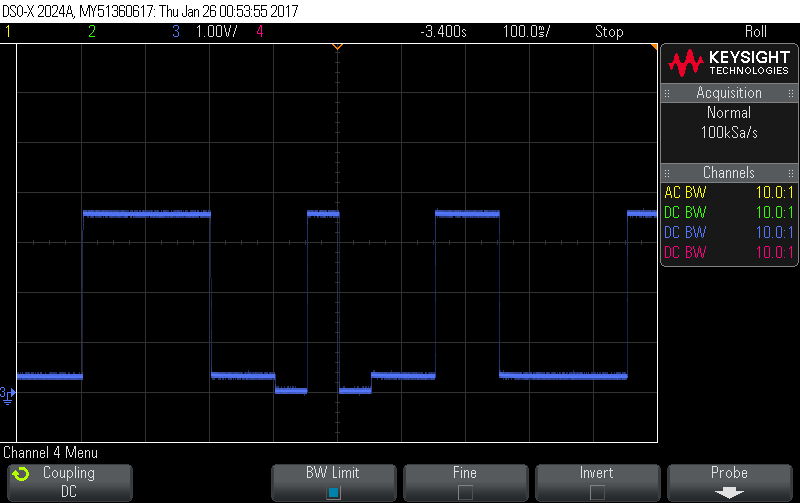
\includegraphics[width=350px]{images/measuring-oscilloscope_ev3-software_led-blinking_part1.png}
	\caption[Zoom na záznam z~osciloskopu po provedení zkušebního programu]{Zoom na záznam z~osciloskopu po provedení zkušebního programu}
	\label{fig:measuring_lego-ev3_orig-soft_led-blinking_part1}
\end{figure}

\begin{figure}[h]
	\centering
	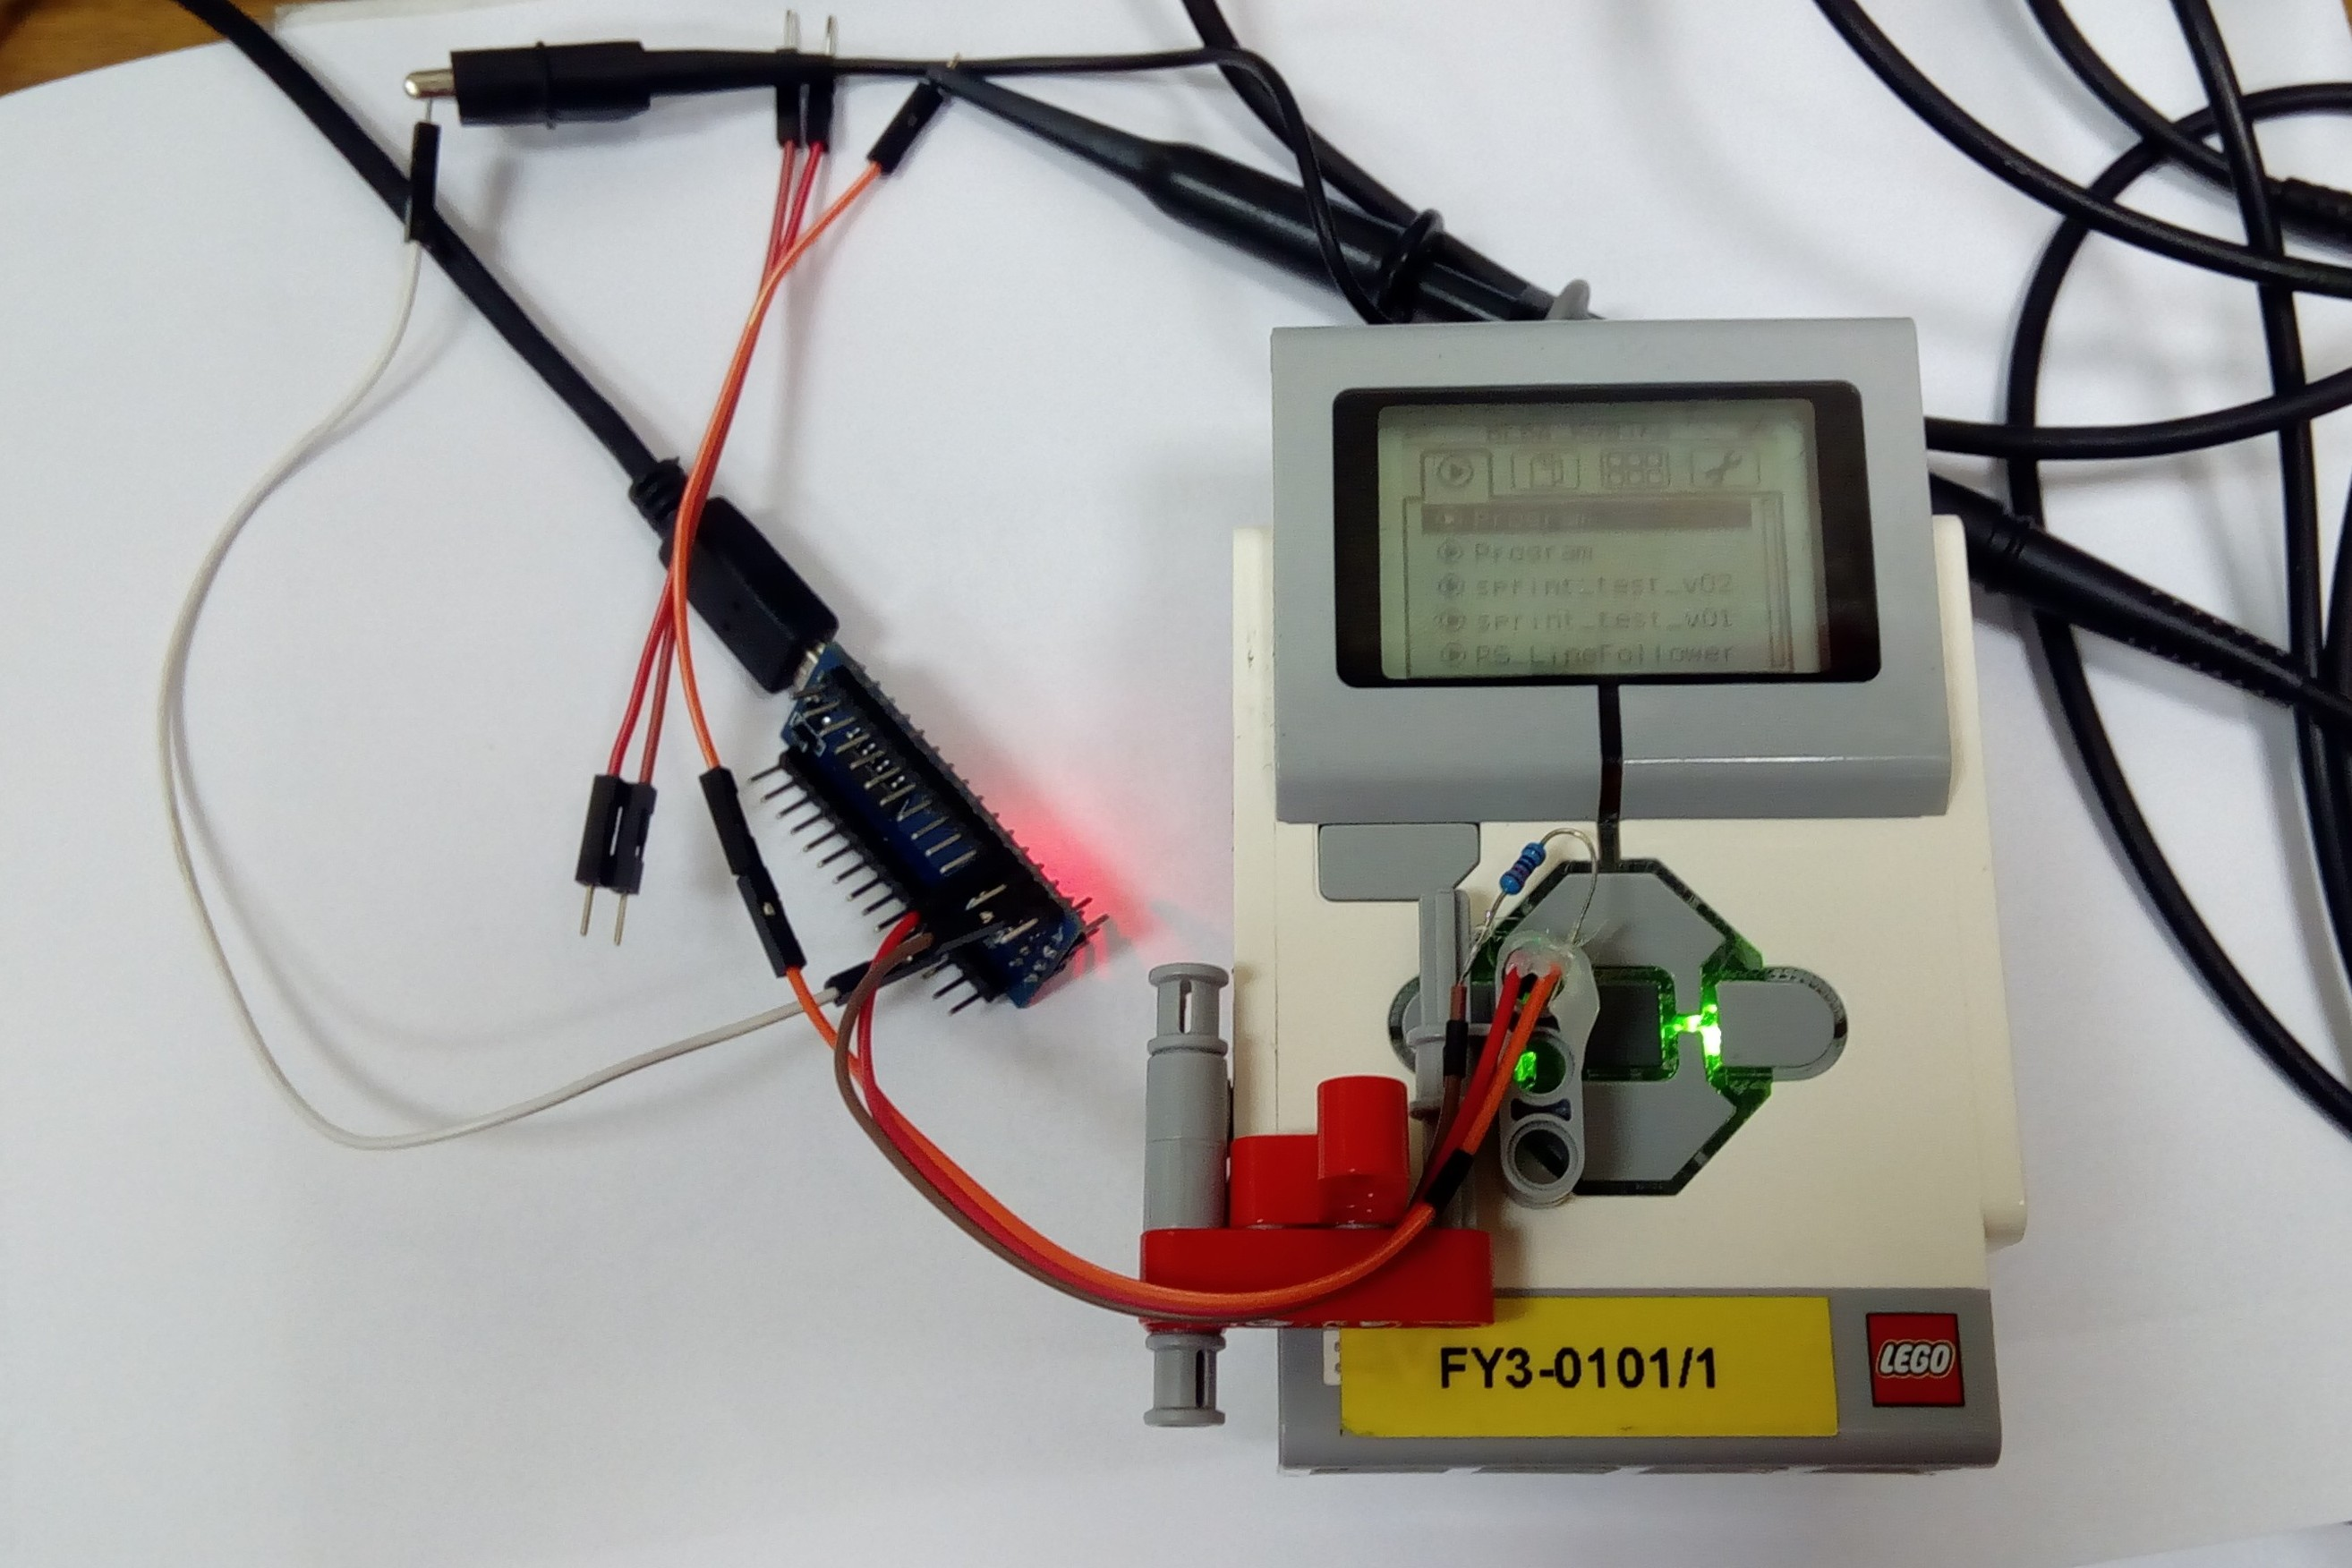
\includegraphics[width=280px]{images/measuring-system_photo.jpg}
	\caption[Foto měřicí sestavy]{Foto měřicí sestavy}
	\label{fig:measuring-system_photo}
\end{figure}

Z~naměřených výsledků vyplývá, že tuto formu testování nelze použít.

\section{Měření jednotlivých operací}

Jelikož nebyli výsledky z~prvního testování uspokojivé, rozhodl jsem se provést testy výkonosti jednotlivých operací na standardním LEGO systému a~RTOS EV3RT (popis v~kapitole \ref{lego-EV3RT}), který dle předchozího zkoumání měl předpoklady k~nejlepšímu výkonu.  \\

V~rámci testů byla vytvořeny dvě sady: 

\begin{itemize}
    \item matematických operací (sčítání, násobení, dělení, \dots) a~podmínka
    \item operace se senzory a~motory
\end{itemize}

Jednotlivé měření se prováděli vícenásobným voláním daných metod (v~rozmezí od~1 do~100~000 volání v~závislosti na době trvání dané operace) tak, aby bylo možné změřit čas s~rozumnou přesností.
Každé měření pak bylo zopakováno 1000, aby bylo možné určit průměr a~maxima. 
Zdrojové soubory k~testům (jak LEGO, tak EV3RT) jsou k~dispozici v~repozitáři RB-ev3rt-hrp2-sdk~\cite{RB-ev3rt-hrp2-sdk-github}.

Matematické operace, jako sčítání, násobení, dělení byly prováděny v~plovoucí desetinné čárce (double).

Z~výkonnostních testu (tabulka~\ref{Benchmark-math} a~\ref{Benchmark-IO}) je dobře vidět, že zpracování operací probíhá na systému EV3RT více jak o~2~řády rychlejší než u~oficiálního systému \EVthree{}. Proto jsem vybral tento systém jako nejvhodnější variantu pro  vytvoření vývojové prostředí.

\begin{table}[h]
\centering

\caption{Porovnání relativního výpočetního výkonu originálního LEGO systému a~EV3RT -- matematické operace a~podmínka \\
}

\label{Benchmark-math}
\begin{tabular}{@{}ccrrr@{}}
\toprule
Označení testu                                       & AVG/MAX                     & LEGO                               & EV3RT                                & Porovnání                                                    \\ \midrule
\multicolumn{1}{|c}{}                                & \cellcolor[HTML]{EFEFEF}AVG & \cellcolor[HTML]{EFEFEF}    563 us & \cellcolor[HTML]{EFEFEF}    0.586 us & \multicolumn{1}{r|}{\cellcolor[HTML]{EFEFEF}    960 $\times$}  \\
\multicolumn{1}{|c}{\multirow{-2}{*}{sčítání}}           & \cellcolor[HTML]{FFFFFF}MAX & \cellcolor[HTML]{FFFFFF}    680 us & \cellcolor[HTML]{FFFFFF}    0.602 us & \multicolumn{1}{r|}{\cellcolor[HTML]{FFFFFF}   1129 $\times$}  \\ \midrule
\multicolumn{1}{|c}{}                                & \cellcolor[HTML]{EFEFEF}AVG & \cellcolor[HTML]{EFEFEF}    388 us & \cellcolor[HTML]{EFEFEF}    0.506 us & \multicolumn{1}{r|}{\cellcolor[HTML]{EFEFEF}    766 $\times$}  \\
\multicolumn{1}{|c}{\multirow{-2}{*}{násobení}}          & \cellcolor[HTML]{FFFFFF}MAX & \cellcolor[HTML]{FFFFFF}    510 us & \cellcolor[HTML]{FFFFFF}    0.526 us & \multicolumn{1}{r|}{\cellcolor[HTML]{FFFFFF}    969 $\times$}  \\ \midrule
\multicolumn{1}{|c}{}                                & \cellcolor[HTML]{EFEFEF}AVG & \cellcolor[HTML]{EFEFEF}    403 us & \cellcolor[HTML]{EFEFEF}    2.627 us & \multicolumn{1}{r|}{\cellcolor[HTML]{EFEFEF}    153 $\times$}  \\
\multicolumn{1}{|c}{\multirow{-2}{*}{dělení}}           & \cellcolor[HTML]{FFFFFF}MAX & \cellcolor[HTML]{FFFFFF}    510 us & \cellcolor[HTML]{FFFFFF}    2.943 us & \multicolumn{1}{r|}{\cellcolor[HTML]{FFFFFF}    173 $\times$}  \\ \midrule
\multicolumn{1}{|c}{}                                & \cellcolor[HTML]{EFEFEF}AVG & \cellcolor[HTML]{EFEFEF}    557 us & \cellcolor[HTML]{EFEFEF}   43.350 us & \multicolumn{1}{r|}{\cellcolor[HTML]{EFEFEF}     12 $\times$}  \\
\multicolumn{1}{|c}{\multirow{-2}{*}{mocnina}}           & \cellcolor[HTML]{FFFFFF}MAX & \cellcolor[HTML]{FFFFFF}   1480 us & \cellcolor[HTML]{FFFFFF}   47.860 us & \multicolumn{1}{r|}{\cellcolor[HTML]{FFFFFF}     30 $\times$}  \\ \midrule
\multicolumn{1}{|c}{}                                & \cellcolor[HTML]{EFEFEF}AVG & \cellcolor[HTML]{EFEFEF}    488 us & \cellcolor[HTML]{EFEFEF}    5.250 us & \multicolumn{1}{r|}{\cellcolor[HTML]{EFEFEF}     92 $\times$}  \\
\multicolumn{1}{|c}{\multirow{-2}{*}{odmocnina}}          & \cellcolor[HTML]{FFFFFF}MAX & \cellcolor[HTML]{FFFFFF}    890 us & \cellcolor[HTML]{FFFFFF}    6.146 us & \multicolumn{1}{r|}{\cellcolor[HTML]{FFFFFF}    144 $\times$}  \\ \midrule
\multicolumn{1}{|c}{}                                & \cellcolor[HTML]{EFEFEF}AVG & \cellcolor[HTML]{EFEFEF}    411 us & \cellcolor[HTML]{EFEFEF}   12.520 us & \multicolumn{1}{r|}{\cellcolor[HTML]{EFEFEF}     32 $\times$}  \\
\multicolumn{1}{|c}{\multirow{-2}{*}{sinus}}           & \cellcolor[HTML]{FFFFFF}MAX & \cellcolor[HTML]{FFFFFF}    590 us & \cellcolor[HTML]{FFFFFF}   15.780 us & \multicolumn{1}{r|}{\cellcolor[HTML]{FFFFFF}     37 $\times$}  \\ \midrule
\multicolumn{1}{|c}{}                                & \cellcolor[HTML]{EFEFEF}AVG & \cellcolor[HTML]{EFEFEF}    419 us & \cellcolor[HTML]{EFEFEF}    0.126 us & \multicolumn{1}{r|}{\cellcolor[HTML]{EFEFEF}   3325 $\times$}  \\
\multicolumn{1}{|c}{\multirow{-2}{*}{podmínka}}     & \cellcolor[HTML]{FFFFFF}MAX & \cellcolor[HTML]{FFFFFF}    510 us & \cellcolor[HTML]{FFFFFF}    0.139 us & \multicolumn{1}{r|}{\cellcolor[HTML]{FFFFFF}   3669 $\times$}  \\ \midrule
\end{tabular}
\end{table}

\begin{table}[]
\centering
\caption{Porovnání relativního výpočetního výkonu originálního LEGO systému a~EV3RT -- \brick{} komponenty, motory a~senzory}
\label{Benchmark-IO}
\begin{tabular}{@{}ccrrr@{}}
\toprule
Označení testu                                       & AVG/MAX                     & LEGO                               & EV3RT                                & Porovnání                                                    \\ \midrule
\multicolumn{1}{|c}{}                                & \cellcolor[HTML]{EFEFEF}AVG & \cellcolor[HTML]{EFEFEF}    966 us & \cellcolor[HTML]{EFEFEF}    0.350 us & \multicolumn{1}{r|}{\cellcolor[HTML]{EFEFEF}   2760 $\times$}  \\
\multicolumn{1}{|c}{\multirow{-2}{*}{brick button}}  & \cellcolor[HTML]{FFFFFF}MAX & \cellcolor[HTML]{FFFFFF}   1100 us & \cellcolor[HTML]{FFFFFF}    0.362 us & \multicolumn{1}{r|}{\cellcolor[HTML]{FFFFFF}   3038 $\times$}  \\ \midrule
\multicolumn{1}{|c}{}                                & \cellcolor[HTML]{EFEFEF}AVG & \cellcolor[HTML]{EFEFEF}    787 us & \cellcolor[HTML]{EFEFEF}    2.866 us & \multicolumn{1}{r|}{\cellcolor[HTML]{EFEFEF}    274 $\times$}  \\
\multicolumn{1}{|c}{\multirow{-2}{*}{brick led}}     & \cellcolor[HTML]{FFFFFF}MAX & \cellcolor[HTML]{FFFFFF}    900 us & \cellcolor[HTML]{FFFFFF}    3.247 us & \multicolumn{1}{r|}{\cellcolor[HTML]{FFFFFF}    277 $\times$}  \\ \midrule
\multicolumn{1}{|c}{}                                & \cellcolor[HTML]{EFEFEF}AVG & \cellcolor[HTML]{EFEFEF}   1449 us & \cellcolor[HTML]{EFEFEF}  396.080 us & \multicolumn{1}{r|}{\cellcolor[HTML]{EFEFEF}      3 $\times$}  \\
\multicolumn{1}{|c}{\multirow{-2}{*}{brick display}} & \cellcolor[HTML]{FFFFFF}MAX & \cellcolor[HTML]{FFFFFF}   1620 us & \cellcolor[HTML]{FFFFFF}  409.330 us & \multicolumn{1}{r|}{\cellcolor[HTML]{FFFFFF}      3 $\times$}  \\ \midrule
\multicolumn{1}{|c}{}                                & \cellcolor[HTML]{EFEFEF}AVG & \cellcolor[HTML]{EFEFEF}    603 us & \cellcolor[HTML]{EFEFEF}    8.770 us & \multicolumn{1}{r|}{\cellcolor[HTML]{EFEFEF}     68 $\times$}  \\
\multicolumn{1}{|c}{\multirow{-2}{*}{motor power}}   & \cellcolor[HTML]{FFFFFF}MAX & \cellcolor[HTML]{FFFFFF}    720 us & \cellcolor[HTML]{FFFFFF}   11.630 us & \multicolumn{1}{r|}{\cellcolor[HTML]{FFFFFF}     61 $\times$}  \\ \midrule
\multicolumn{1}{|c}{}                                & \cellcolor[HTML]{EFEFEF}AVG & \cellcolor[HTML]{EFEFEF}    612 us & \cellcolor[HTML]{EFEFEF}    8.840 us & \multicolumn{1}{r|}{\cellcolor[HTML]{EFEFEF}     69 $\times$}  \\
\multicolumn{1}{|c}{\multirow{-2}{*}{motor speed}}   & \cellcolor[HTML]{FFFFFF}MAX & \cellcolor[HTML]{FFFFFF}    760 us & \cellcolor[HTML]{FFFFFF}   11.670 us & \multicolumn{1}{r|}{\cellcolor[HTML]{FFFFFF}     65 $\times$}  \\ \midrule
\multicolumn{1}{|c}{}                                & \cellcolor[HTML]{EFEFEF}AVG & \cellcolor[HTML]{EFEFEF}   1023 us & \cellcolor[HTML]{EFEFEF}   17.490 us & \multicolumn{1}{r|}{\cellcolor[HTML]{EFEFEF}     58 $\times$}  \\
\multicolumn{1}{|c}{\multirow{-2}{*}{motors speed}}  & \cellcolor[HTML]{FFFFFF}MAX & \cellcolor[HTML]{FFFFFF}   1160 us & \cellcolor[HTML]{FFFFFF}   21.120 us & \multicolumn{1}{r|}{\cellcolor[HTML]{FFFFFF}     54 $\times$}  \\ \midrule
\multicolumn{1}{|c}{}                                & \cellcolor[HTML]{EFEFEF}AVG & \cellcolor[HTML]{EFEFEF}    785 us & \cellcolor[HTML]{EFEFEF}    3.870 us & \multicolumn{1}{r|}{\cellcolor[HTML]{EFEFEF}    202 $\times$}  \\
\multicolumn{1}{|c}{\multirow{-2}{*}{CS reflected}}  & \cellcolor[HTML]{FFFFFF}MAX & \cellcolor[HTML]{FFFFFF}    940 us & \cellcolor[HTML]{FFFFFF}    6.980 us & \multicolumn{1}{r|}{\cellcolor[HTML]{FFFFFF}    134 $\times$}  \\ \midrule
\multicolumn{1}{|c}{}                                & \cellcolor[HTML]{EFEFEF}AVG & \cellcolor[HTML]{EFEFEF}    830 us & \cellcolor[HTML]{EFEFEF}    3.860 us & \multicolumn{1}{r|}{\cellcolor[HTML]{EFEFEF}    215 $\times$}  \\
\multicolumn{1}{|c}{\multirow{-2}{*}{CS ambient}}    & \cellcolor[HTML]{FFFFFF}MAX & \cellcolor[HTML]{FFFFFF}    990 us & \cellcolor[HTML]{FFFFFF}    7.100 us & \multicolumn{1}{r|}{\cellcolor[HTML]{FFFFFF}    139 $\times$}  \\ \midrule
\multicolumn{1}{|c}{}                                & \cellcolor[HTML]{EFEFEF}AVG & \cellcolor[HTML]{EFEFEF}    799 us & \cellcolor[HTML]{EFEFEF}    3.890 us & \multicolumn{1}{r|}{\cellcolor[HTML]{EFEFEF}    205 $\times$}  \\
\multicolumn{1}{|c}{\multirow{-2}{*}{CS color}}      & \cellcolor[HTML]{FFFFFF}MAX & \cellcolor[HTML]{FFFFFF}    930 us & \cellcolor[HTML]{FFFFFF}    6.730 us & \multicolumn{1}{r|}{\cellcolor[HTML]{FFFFFF}    138 $\times$}  \\ \midrule
\multicolumn{1}{|c}{}                                & \cellcolor[HTML]{EFEFEF}AVG & \cellcolor[HTML]{EFEFEF}    811 us & \cellcolor[HTML]{EFEFEF}    3.841 us & \multicolumn{1}{r|}{\cellcolor[HTML]{EFEFEF}    211 $\times$}  \\
\multicolumn{1}{|c}{\multirow{-2}{*}{UTS cm}}        & \cellcolor[HTML]{FFFFFF}MAX & \cellcolor[HTML]{FFFFFF}    960 us & \cellcolor[HTML]{FFFFFF}    4.212 us & \multicolumn{1}{r|}{\cellcolor[HTML]{FFFFFF}    227 $\times$}  \\ \midrule
\multicolumn{1}{|c}{}                                & \cellcolor[HTML]{EFEFEF}AVG & \cellcolor[HTML]{EFEFEF}    827 us & \cellcolor[HTML]{EFEFEF}    3.838 us & \multicolumn{1}{r|}{\cellcolor[HTML]{EFEFEF}    215 $\times$}  \\
\multicolumn{1}{|c}{\multirow{-2}{*}{UTS inch}}      & \cellcolor[HTML]{FFFFFF}MAX & \cellcolor[HTML]{FFFFFF}   1030 us & \cellcolor[HTML]{FFFFFF}    4.197 us & \multicolumn{1}{r|}{\cellcolor[HTML]{FFFFFF}    245 $\times$}  \\ \midrule
\multicolumn{1}{|c}{}                                & \cellcolor[HTML]{EFEFEF}AVG & \cellcolor[HTML]{EFEFEF}    845 us & \cellcolor[HTML]{EFEFEF}    3.769 us & \multicolumn{1}{r|}{\cellcolor[HTML]{EFEFEF}    224 $\times$}  \\
\multicolumn{1}{|c}{\multirow{-2}{*}{UTS listen}}    & \cellcolor[HTML]{FFFFFF}MAX & \cellcolor[HTML]{FFFFFF}   1220 us & \cellcolor[HTML]{FFFFFF}    4.115 us & \multicolumn{1}{r|}{\cellcolor[HTML]{FFFFFF}    296 $\times$}  \\ \midrule
\multicolumn{1}{|c}{}                                & \cellcolor[HTML]{EFEFEF}AVG & \cellcolor[HTML]{EFEFEF}    851 us & \cellcolor[HTML]{EFEFEF}    3.910 us & \multicolumn{1}{r|}{\cellcolor[HTML]{EFEFEF}    217 $\times$}  \\
\multicolumn{1}{|c}{\multirow{-2}{*}{GYRO angle}}    & \cellcolor[HTML]{FFFFFF}MAX & \cellcolor[HTML]{FFFFFF}   1050 us & \cellcolor[HTML]{FFFFFF}    6.740 us & \multicolumn{1}{r|}{\cellcolor[HTML]{FFFFFF}    155 $\times$}  \\ \midrule
\multicolumn{1}{|c}{}                                & \cellcolor[HTML]{EFEFEF}AVG & \cellcolor[HTML]{EFEFEF}    847 us & \cellcolor[HTML]{EFEFEF}    3.920 us & \multicolumn{1}{r|}{\cellcolor[HTML]{EFEFEF}    216 $\times$}  \\
\multicolumn{1}{|c}{\multirow{-2}{*}{GYRO rate}}     & \cellcolor[HTML]{FFFFFF}MAX & \cellcolor[HTML]{FFFFFF}   1250 us & \cellcolor[HTML]{FFFFFF}    7.190 us & \multicolumn{1}{r|}{\cellcolor[HTML]{FFFFFF}    173 $\times$}  \\ \midrule
\multicolumn{1}{|c}{}                                & \cellcolor[HTML]{EFEFEF}AVG & \cellcolor[HTML]{EFEFEF}  25712 us & \cellcolor[HTML]{EFEFEF}    3.510 us & \multicolumn{1}{r|}{\cellcolor[HTML]{EFEFEF}   7325 $\times$}  \\
\multicolumn{1}{|c}{\multirow{-2}{*}{GYRO reset}}    & \cellcolor[HTML]{FFFFFF}MAX & \cellcolor[HTML]{FFFFFF}  34410 us & \cellcolor[HTML]{FFFFFF}    6.420 us & \multicolumn{1}{r|}{\cellcolor[HTML]{FFFFFF}   5359 $\times$}  \\ \midrule
\end{tabular}
\end{table}


  
  \chapter{Osnova práce}
\section{Úvod}
\section{Historie LEGO MINDSTORMS}
\section{Dostupné platformy pro programování EV3}
\section{?Testování platforem}
\section{EV3RT}
\section{Rozvoj EV3RT}
\section{Závěr}
    	
  % Pouzita literatura / Bibliography
  % ----------------------------------------------
\ifslovak
  \makeatletter
  \def\@openbib@code{\addcontentsline{toc}{chapter}{Literatúra}}
  \makeatother
  \bibliographystyle{bib-styles/czechiso}
\else
  \ifczech
    \makeatletter
    \def\@openbib@code{\addcontentsline{toc}{chapter}{Literatura}}
    \makeatother
    \bibliographystyle{bib-styles/czechiso}
  \else 
    \makeatletter
    \def\@openbib@code{\addcontentsline{toc}{chapter}{Bibliography}}
    \makeatother
    \bibliographystyle{bib-styles/englishiso}
  %  \bibliographystyle{alpha}
  \fi
\fi
  \begin{flushleft}
  \bibliography{projekt-20-literatura-bibliography}
  \end{flushleft}

  % vynechani stranky v oboustrannem rezimu
  % Skip the page in the two-sided mode
  \iftwoside
    \cleardoublepage
  \fi

  % Prilohy / Appendices
  % ---------------------------------------------
  \appendix
\ifczech
  \renewcommand{\appendixpagename}{Přílohy}
  \renewcommand{\appendixtocname}{Přílohy}
  \renewcommand{\appendixname}{Příloha}
\fi
\ifslovak
  \renewcommand{\appendixpagename}{Prílohy}
  \renewcommand{\appendixtocname}{Prílohy}
  \renewcommand{\appendixname}{Príloha}
\fi
%  \appendixpage

% vynechani stranky v oboustrannem rezimu
% Skip the page in the two-sided mode
%\iftwoside
%  \cleardoublepage
%\fi
  
\ifslovak
%  \section*{Zoznam príloh}
%  \addcontentsline{toc}{section}{Zoznam príloh}
\else
  \ifczech
%    \section*{Seznam příloh}
%    \addcontentsline{toc}{section}{Seznam příloh}
  \else
%    \section*{List of Appendices}
%    \addcontentsline{toc}{section}{List of Appendices}
  \fi
\fi
  \startcontents[chapters]
  \setlength{\parskip}{0pt}
  % seznam příloh / list of appendices
  % \printcontents[chapters]{l}{0}{\setcounter{tocdepth}{2}}
  
  \ifODSAZ
    \setlength{\parskip}{0.5\bigskipamount}
  \else
    \setlength{\parskip}{0pt}
  \fi
  
  % vynechani stranky v oboustrannem rezimu
  \iftwoside
    \cleardoublepage
  \fi
  %\chapter{Obrázky}

\begin{figure}[h]
	\centering
	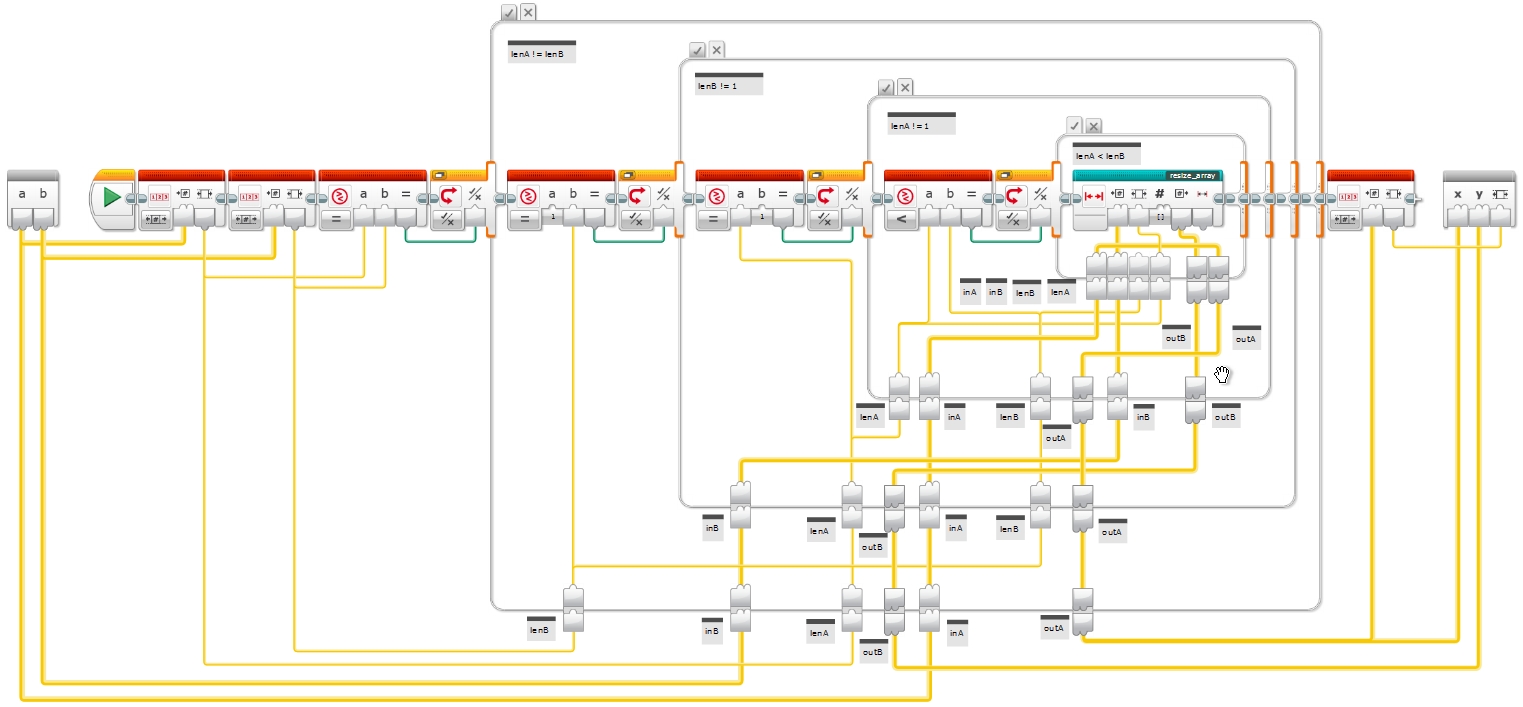
\includegraphics[angle=-90,origin=c,width=280px]{images/lego-soft_legolib_match_array_length.png}
	\caption[Předávání hodnot v \legoSW{}]{Předávání hodnot v \legoSW{}}
	\label{fig:lego-soft_legolib_match_array_length}
\end{figure}




 % viz. prilohy.tex / see prilohy.tex
\end{document}
